\documentclass[12pt,]{article}
\usepackage{lmodern}
\usepackage{amssymb,amsmath}
\usepackage{ifxetex,ifluatex}
\usepackage{fixltx2e} % provides \textsubscript
\ifnum 0\ifxetex 1\fi\ifluatex 1\fi=0 % if pdftex
  \usepackage[T1]{fontenc}
  \usepackage[utf8]{inputenc}
\else % if luatex or xelatex
  \ifxetex
    \usepackage{mathspec}
  \else
    \usepackage{fontspec}
  \fi
  \defaultfontfeatures{Ligatures=TeX,Scale=MatchLowercase}
\fi
% use upquote if available, for straight quotes in verbatim environments
\IfFileExists{upquote.sty}{\usepackage{upquote}}{}
% use microtype if available
\IfFileExists{microtype.sty}{%
\usepackage{microtype}
\UseMicrotypeSet[protrusion]{basicmath} % disable protrusion for tt fonts
}{}
\usepackage[margin=1in]{geometry}
\usepackage{hyperref}
\hypersetup{unicode=true,
            pdfborder={0 0 0},
            breaklinks=true}
\urlstyle{same}  % don't use monospace font for urls
\usepackage{longtable,booktabs}
\usepackage{graphicx,grffile}
\makeatletter
\def\maxwidth{\ifdim\Gin@nat@width>\linewidth\linewidth\else\Gin@nat@width\fi}
\def\maxheight{\ifdim\Gin@nat@height>\textheight\textheight\else\Gin@nat@height\fi}
\makeatother
% Scale images if necessary, so that they will not overflow the page
% margins by default, and it is still possible to overwrite the defaults
% using explicit options in \includegraphics[width, height, ...]{}
\setkeys{Gin}{width=\maxwidth,height=\maxheight,keepaspectratio}
\IfFileExists{parskip.sty}{%
\usepackage{parskip}
}{% else
\setlength{\parindent}{0pt}
\setlength{\parskip}{6pt plus 2pt minus 1pt}
}
\setlength{\emergencystretch}{3em}  % prevent overfull lines
\providecommand{\tightlist}{%
  \setlength{\itemsep}{0pt}\setlength{\parskip}{0pt}}
\setcounter{secnumdepth}{5}
% Redefines (sub)paragraphs to behave more like sections
\ifx\paragraph\undefined\else
\let\oldparagraph\paragraph
\renewcommand{\paragraph}[1]{\oldparagraph{#1}\mbox{}}
\fi
\ifx\subparagraph\undefined\else
\let\oldsubparagraph\subparagraph
\renewcommand{\subparagraph}[1]{\oldsubparagraph{#1}\mbox{}}
\fi

%%% Use protect on footnotes to avoid problems with footnotes in titles
\let\rmarkdownfootnote\footnote%
\def\footnote{\protect\rmarkdownfootnote}

%%% Change title format to be more compact
\usepackage{titling}

% Create subtitle command for use in maketitle
\newcommand{\subtitle}[1]{
  \posttitle{
    \begin{center}\large#1\end{center}
    }
}

\setlength{\droptitle}{-2em}
  \title{}
  \pretitle{\vspace{\droptitle}}
  \posttitle{}
  \author{}
  \preauthor{}\postauthor{}
  \date{}
  \predate{}\postdate{}


\begin{document}

{
\setcounter{tocdepth}{2}
\tableofcontents
}
\hypertarget{description-courte-a-publier}{%
\section{1. Description courte à
publier}\label{description-courte-a-publier}}

Madagascar est une île de l'océan indien qui s'est détachée de l'Afrique
puis de l'Inde il y a plusieurs dizaines de millions d'années. La
biodiversité y a évolué de façon isolée. Ainsi, près de 90\% des espèces
n'existent que sur l'île. Cette biodiversité est fortement menacée par
les changements climatiques et la déforestation. Le projet BioSceneMada,
en s'appuyant sur des modèles climatiques, écologiques et paysagers, se
propose d'établir des scénarios d'évolution de la biodiversité à
Madagascar sous l'effet conjoint du changement climatique et de la
déforestation. Les cartes issues du projet permettent d'identifier les
zones à risque de perte de biodiversité et de déforestation ainsi que
les zones refuges pour la biodiversité. Ces cartes peuvent être
utilisées afin d'agir efficacement pour la conservation des forêts et de
la biodiversité à Madagascar, notamment en priorisant les actions de
conservation sur des zones cibles, tout en s'appuyant sur le réseau
d'aires protégées actuel.






\begin{figure}[H]

{\centering 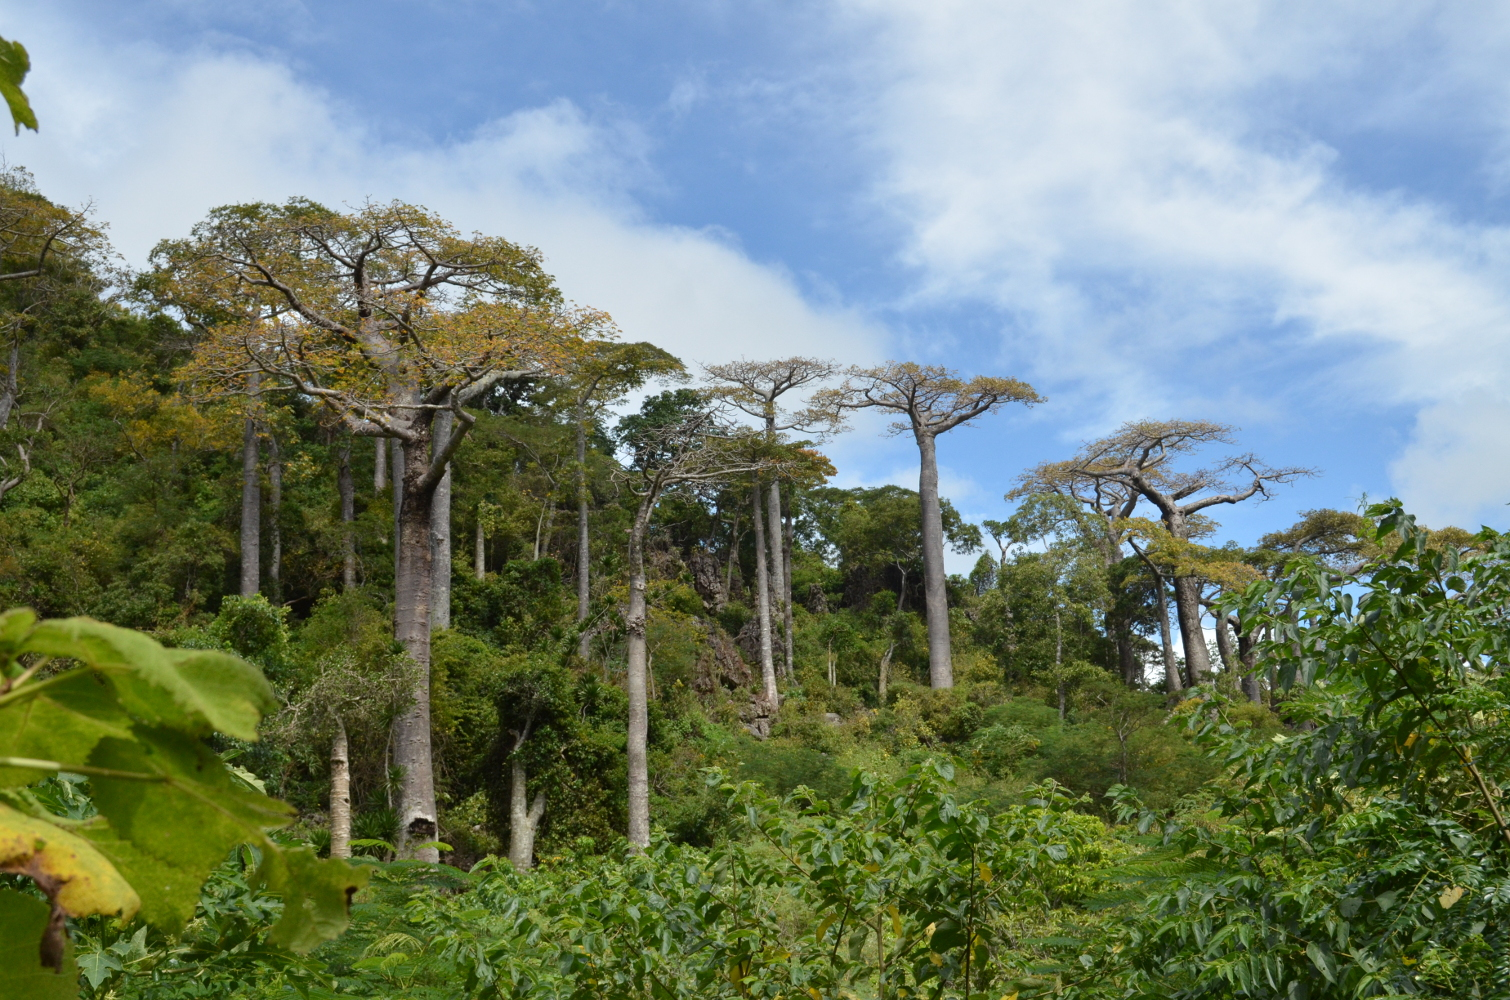
\includegraphics[width=\textwidth]{figures/Adansonia_suarezensis} 

}

\caption{\textbf{Population de baobabs de l'espèce
\emph{Adansonia suarezensis} sur le site de la Montagne des Français au
nord de Madagascar.} Cette espèce est fortement menacée par la perte
d'habitat associée aux changements climatiques.}\label{fig:baobab}
\end{figure}





\begin{figure}[H]

{\centering 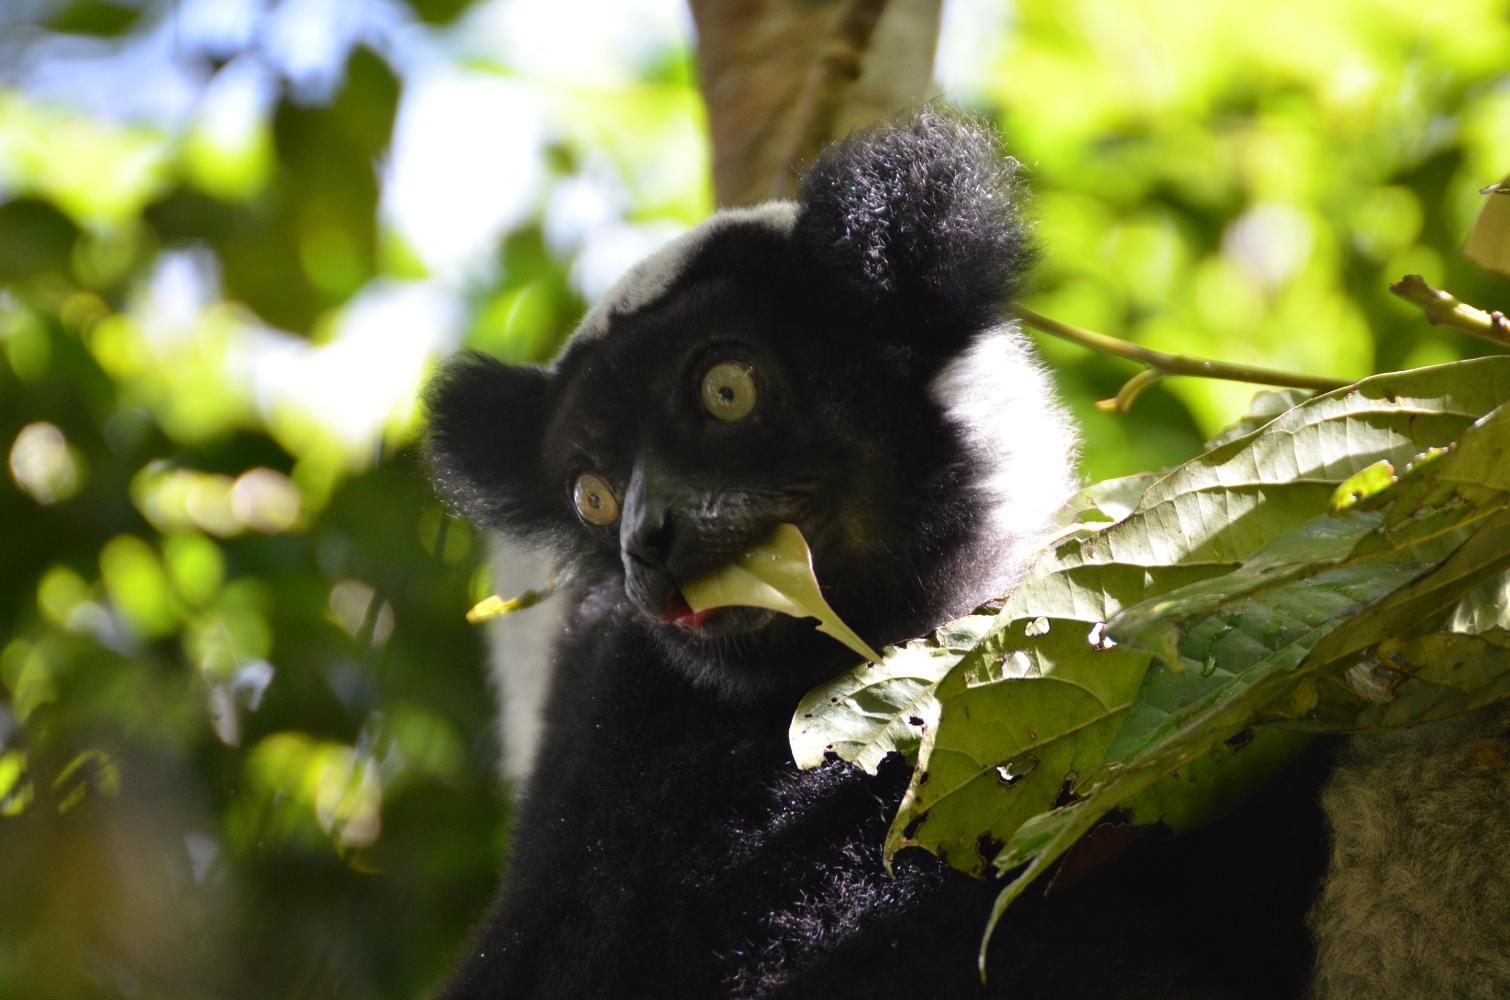
\includegraphics[width=\textwidth]{figures/Indri_indri} 

}

\caption{\textbf{Lémurien de l'espèce \emph{Indri indri} dans le
parc national de Mantadia à l'est de Madagascar.} Cette espèce est
fortement menacée par la perte d'habitat associée à la déforestation.}\label{fig:lemur}
\end{figure}

\hypertarget{resume}{%
\section{2. Résumé}\label{resume}}

Le projet FRB-FFEM BioSceneMada vise à produire des scénarios
d'évolution de la biodiversité à Madagascar sous l'effet conjoint du
changement climatique et de la déforestation d'origine anthropique
(\url{https://bioscenemada.cirad.fr}). Le projet a une durée de 60 mois
(36 mois consacrés au travail de recherche et 24 mois consacrés au
transfert et à la communication des résultats auprès des gestionnaires
de la biodiversité à Madagascar et des décideurs politiques). Démarré
courant 2014, il se terminera en 2019. Le projet associe quatre
partenaires en France (Cirad, ETC Terra) et à Madagascar (WCS
Madagascar, Office National de l'Environnement).

Madagascar est reconnu pour son exceptionnelle biodiversité, tant du
point de vue du nombre d'espèces que des taux d'endémisme (proches de
90\% dans tous les groupes taxonomiques). Cette biodiversité,
principalement concentrée dans les forêts tropicales de l'île, est
sévèrement menacée par le changement climatique et la déforestation.
L'objectif du projet BioSceneMada est premièrement d'établir des
scénarios de déforestation (en tenant compte notamment de la croissance
démographique) et d'estimer la perte de biodiversité associée à ces
scénarios. Deuxièmement, l'objectif est d'estimer l'impact des
changements climatiques sur la perte de biodiversité. L'impact sur la
biodiversité sera considéré sous l'angle des espèces (risque
d'extinction des espèces via la restriction des aires de distribution,
ex. les espèces de baobabs) mais également sous l'angle des communautés
(perte d'habitat ou restriction des habitats pour les communautés, ex.
la forêt épineuse). Troisièmement, l'objectif du projet est d'identifier
les futurs points-chauds (``hotspots'') de biodiversité à fort risque de
déforestation. Ces scénarios permettront notamment de réfléchir à
l'optimisation du réseau d'aires naturelles protégées en concentrant les
efforts de conservation sur des zones cibles identifiées sur la base de
résultats scientifiques.

Les premiers résultats de recherche ont permis de proposer des scénarios
de référence pour la déforestation à Madagascar à l'horizon 2050 et
2100. En s'appuyant sur l'étude de la déforestation passée (période
1990-2000-2010), les modèles prédisent une diminution du couvert
forestier de 9.3 millions d'hectares (Mha) en 2010 à environ 5 Mha en
2050 et moins de 2 Mha en 2100. La déforestation se fait majoritairement
en dehors des aires protégées jusqu'en 2050, puis pénètre dans les aires
protégées au-delà de cette date. En 2100, la forêt résiduelle se situe
en altitude dans des zones reculées (péninsule de Masoala).

Une base regroupant les données d'occurrence de 4969 espèces a également
été constituée. Cette base regroupe des données animales (vertébrés et
invertébrés) et végétales (arbres et autres plantes) pour une grande
variété de groupes taxonomiques, représentatifs de la biodiversité à
Madagascar. Cette base constitue un inventaire sans précédent de la
biodiversité à Madagascar et regoupe des données vérifiées tant du point
de vue taxonomique que de la localisation géographique. Ces données ont
été utilisées pour modéliser la niche climatique des espèces et estimer
leur vulnérabilité aux changements climatique. Les données issues des
modèles climatiques du GIEC pour Madagascar ont été regroupées sur le
site MadaClim (\url{https://madaclim.cirad.fr}) qui est un des produits
du projet BioSceneMada. Un atlas comprenant les aires de distribution
présentes et futures de l'ensemble des 4969 espèces sera édité. Cette
analyse permettra d'identifier les hotspots présents et futurs de la
biodiversité. A l'échelle de la communauté, ces données ont également
été utilisées pour mettre en évidence l'effet du climat sur la structure
des communautés. On montre notamment que l'importance du climat dans la
détermination de l'assemblage des espèces est très variable d'un groupe
taxonomique à l'autre.

Les résultats du projet montrent également que les forêts humides se
situant en altitude, dans les zones peu acessibles (péninsule de Masoala
notamment), et qui seront impactées tardivement par la déforestation,
sont les plus sensibles au changement climatique. Les espèces de ces
forêts sont en effet peu adaptées à une augmentation forte de la
saisonnalité (impliquant une diminution de la saison de végétation) et à
une augmentation forte de la température prévues dans cette région.
Ainsi, la conservation de la forêt et de la biodiversité à Madagascar
face à la double contrainte de la déforestation et du changement
climatique constitue un véritable challenge. Au vue de ces résultats, la
première action à entreprendre nous semble de lutter efficacement contre
la déforestation afin de conserver les forêts naturelles existantes, qui
ne représentent que 15\% du territoire national à Madagascar en 2014.
Nos résultats montrent également que ces actions de conservation ne
pourront se mettre en place à Madagascar sans une meilleure orientation
de l'aide internationale au développement avec pour objectif une
amélioration de la gouvernance, une lutte contre la corruption et
l'application des lois environnementales.

\hypertarget{vos-principaux-resultats-valorises-dans-les-publications-scientifiques}{%
\section{3. Vos principaux résultats valorisés dans les publications
scientifiques}\label{vos-principaux-resultats-valorises-dans-les-publications-scientifiques}}

\hypertarget{madaclim-portail-de-donnees-climatiques-et-environnementales-a-madagascar}{%
\subsection{MadaClim: portail de données climatiques et
environnementales à
Madagascar}\label{madaclim-portail-de-donnees-climatiques-et-environnementales-a-madagascar}}

Nous avons développé le site internet MadaClim
(\url{https://madaclim.cirad.fr} qui reprend toutes les données
climatiques actuelles ainsi que les prédictions climatiques issues des
modèles du GIEC (groupe d'experts intergouvernemental sur l'évolution du
climat). Les données sont à 1km de résolution et distribuées
spécifiquement pour Madagascar. Des variables bioclimatiques comme
l'évapotranspiration et le nombre de mois secs ont été recalculées et
ajoutées aux variables existantes. En plus des données climatiques, des
données environnementales incluant altitude, pente, irradiation solaire,
géologie, sol, etc. ont été compilées.

\emph{Référence:}

Vieilledent G., O. Gardi, C. Grinand, C. Burren, M. Andriamanjato, C.
Camara, C. J. Gardner, L. Glass, A. Rasolohery, H. Rakoto Ratsimba, V.
Gond, and J.-R. Rakotoarijaona. 2016. Bioclimatic envelope models
predict a decrease in tropical forest carbon stocks with climate change
in Madagascar. \emph{Journal of Ecology}. 104: 703-715. doi:
\url{https://doi.org/10.1111/1365-2745.12548}.

Vieilledent G. 2016. MadaClim: a set of climatic and environmental
spatial variables for Madagascar. Data paper. in prep.

\hypertarget{carte-de-carbone-forestier-et-vulnerabilite-des-forets-tropicales-au-changement-climatique-a-madagascar}{%
\subsection{Carte de carbone forestier et vulnérabilité des forêts
tropicales au changement climatique à
Madagascar}\label{carte-de-carbone-forestier-et-vulnerabilite-des-forets-tropicales-au-changement-climatique-a-madagascar}}

En utilisant les données climatiques précédemment calculées
(\url{https://madaclim.cirad.fr}) et des données d'inventaires
forestiers pour 1771 placettes réparties sur l'ensemble de Madagascar,
nous avons démontré qu'il existait un lien fort entre climat et stocks
de carbone forestiers. Nous avons produit une carte précise des stocks
de carbone forestier en 2010 à Madagascar à une résolution de 250 m. Les
changements climatiques devraient induire des modifications fortes des
communautés forestières et en conséquence une diminution de -17\%
(7-24\%) des stocks de carbone forestier à Madagascar à l'horizon 2100
par rapport à 2010.

\emph{Références:}

Vieilledent G., O. Gardi, C. Grinand, C. Burren, M. Andriamanjato, C.
Camara, C. J. Gardner, L. Glass, A. Rasolohery, H. Rakoto Ratsimba, V.
Gond, and J.-R. Rakotoarijaona. 2016. Bioclimatic envelope models
predict a decrease in tropical forest carbon stocks with climate change
in Madagascar. \emph{Journal of Ecology}. 104: 703-715. doi:
\url{https://doi.org/10.1111/1365-2745.12548}.

El Hajj M., N. Baghdadi, I. Fayad, G. Vieilledent, J.-S. Bailly, and D.
Ho Tong Minh. 2017. Interest of integrating spaceborne LiDAR data to
improve the estimation of biomass in high biomass forested areas.
\emph{Remote Sensing}. 9(3). \url{https://doi.org/10.3390/rs9030213}.

\hypertarget{base-de-donnees-de-biodiversite-a-madagascar}{%
\subsection{Base de données de biodiversité à
Madagascar}\label{base-de-donnees-de-biodiversite-a-madagascar}}

Nous avons construit un jeu de données sur la biodiversité à Madagascar
regroupant 300 000 observations (points de présence) pour 4969 espèces.
Ces espèces sont réparties dans différents groupes taxonomiques
(Plantes, Vertébrés, Invertébrés) et sont représentatives de la
biodiversité à Madagascar. Ces données, provenant de différents
instituts, sont issues d'un travail de prospection conséquent qui
s'étalent sur plusieurs dizaines d'années.

\emph{Référence:}

Charra M., S. Goodman, A. Raselimanana, M.-J. Raherilalao, V.
Soarimalala, D. Lees, F. Rakotondrainibe, J. Moat, M. Andriamanjato, W.
J. Baker, M. Rakotoarinivo, M. Vorontsova, T. Pearce, T. F. Allnutt, D.
Razafimpahanana, M. Pedrono, J.-R. Rakotoarijaona and G. Vieilledent.
Climate or watersheds ? Environmental factors determining species
assemblages change according to the taxonomic group. in prep.

\hypertarget{atlas-de-la-biodiversite-a-madagascar-et-de-sa-vulnerabilite-au-changement-climatique}{%
\subsection{Atlas de la biodiversité à Madagascar et de sa vulnérabilité
au changement
climatique}\label{atlas-de-la-biodiversite-a-madagascar-et-de-sa-vulnerabilite-au-changement-climatique}}

Nous avons développé un script \texttt{R} permettant de modéliser la
niche climatique des espèces à partir de modèles d'ensemble (Vieilledent
et al. 2013; Araujo and New 2007). Le script permet d'estimer l'aire de
distribution actuelle et future des espèces à Madagascar. En utilisant
cette approche pour les 4969 espèces du jeu de données sur la
biodiversité à Madagascar, l'idée est d'obtenir un atlas de la
biodiversité à Madagascar et de sa vulnérabilité au changement
climatique. Un prototype de cet atlas a été réalisé pour les 7 espèces
de baobab présentes à Madagascar.

\emph{Référence:}

Muniz-Tagliari M., J.-M. Leong Pock-Tsy, C. Cornu and P. Danthu and G.
Vieilledent. Vulnerability of the seven baobab species in Madagascar to
climate change. in prep.

Vieilledent G., M. Muniz-Tagliari, C. Grinand, F. Montfort. Atlas of the
biodiversity of Madagascar: present species distribution and species
vulnerability to climate change. in prep.

\hypertarget{cartes-de-biodiversite-et-des-communautes-despeces-a-madagascar}{%
\subsection{Cartes de biodiversité et des communautés d'espèces à
Madagascar}\label{cartes-de-biodiversite-et-des-communautes-despeces-a-madagascar}}

En utilisant des modèles de communautés (Ferrier et al. 2007), nous
avons cherché à identifier les facteurs environnementaux déterminants
les assemblages d'espèces. Ces facteurs peuvent être climatiques ou
associés à des barrières géographiques comme les bassins versants ou les
rivières (Pearson and Raxworthy 2009). En appliquant ce modèle à nos
données de présence d'espèces à Madagascar, nous avons obtenu une
première carte de la biodiversité \(\beta\) à Madagascar. Mais le
pourcentage de déviance expliquée par le modèle est faible
(\textless{}10\%). En applicant ce même modèle à chaque groupe
taxonomique, nous avons trouvé que les facteurs explicants l'assemblage
des communautés d'espèces variaient d'un groupe taxonomique à l'autre,
le climat n'étant pas toujours le facteur le plus important. Pour le
groupe des lémuriens, ce sont les bassins versants qui expliquent en
majorité l'assemblage des espèces. A contrario, le climat explique une
grande partie des assemblages d'espèces de reptiles et d'amphibiens,
espèces poïkilothermes (animaux ayant une température corporelle qui
varie avec celle de leur milieu). Pour d'autres groupes, comme les
arbres, les facteurs climatiques et les bassins versants semblent
expliquer à part égale les assemblages d'espèces.

\emph{Référence:}

Charra M., S. Goodman, A. Raselimanana, M.-J. Raherilalao, V.
Soarimalala, D. Lees, F. Rakotondrainibe, J. Moat, M. Andriamanjato, W.
J. Baker, M. Rakotoarinivo, M. Vorontsova, T. Pearce, T. F. Allnutt, D.
Razafimpahanana, M. Pedrono, J.-R. Rakotoarijaona and G. Vieilledent.
Climate or watersheds? Environmental factors determining species
assemblages change according to the taxonomic group. in prep.

\hypertarget{soixante-ans-1953-2014-detude-de-la-deforestation-et-de-la-fragmentation-forestiere-a-madagascar}{%
\subsection{Soixante ans (1953-2014) d'étude de la déforestation et de
la fragmentation forestière à
Madagascar}\label{soixante-ans-1953-2014-detude-de-la-deforestation-et-de-la-fragmentation-forestiere-a-madagascar}}

Nous avons obtenu de nouvelles cartes d'évolution de la couverture
forestière à Madagascar sur la période 2000-2014. Elles viennent
compléter les cartes de G. J. Harper et al. (2007) pour les années 1953,
1973 et 1990. Nous montrons que le couvert forestier a diminué de 44\%
sur la période 1953-2014. Les forêts naturelles couvrent 8.9 Mha en 2014
(15\% du territoire national) et incluent 4.4 Mha (50\%) de forêt
humide, 2.6 Mha (29\%) de forêt sèche, 1.7 Mha de forêt épineuse (19\%)
et environ 177,000 ha (2\%) de mangrove. Depuis 2005, les surfaces
déforestées annuellement ont augmenté à Madagascar pour atteindre 100
000 ha/an sur la période 2010-2014. Aujourd'hui, environ 50\% de la
forêt est située à moins de 100 m de la lisière et est donc exposée aux
perturbations.

\emph{Référence:}

Vieilledent G., C. Grinand, F. A. Rakotomalala, R. Ranaivosoa, J.-R.
Rakotoarijaona, T. F. Allnutt, and F. Achard. Combining global tree
cover loss data with historical national forest-cover maps to look at
six decades of deforestation and forest fragmentation in Madagascar.
\emph{bioRxiv}. 147827. doi: \url{https://doi.org/10.1101/147827}. in
review in \emph{Biological Conservation}.

\hypertarget{retour-sur-les-facteurs-de-deforestation-la-pauvrete-nest-pas-lunique-responsable-de-la-deforestation-a-madagascar.}{%
\subsection{Retour sur les facteurs de déforestation: la pauvreté n'est
pas l'unique responsable de la déforestation à
Madagascar.}\label{retour-sur-les-facteurs-de-deforestation-la-pauvrete-nest-pas-lunique-responsable-de-la-deforestation-a-madagascar.}}

A l'issue d'une mission de terrain dans le Menabe, à l'ouest de
Madagascar, nous avons conclu que les causes directes de la
déforestation dans la région sont l'agriculture sur brulis pour la
culture de rente comme le maïs ou l'arachide. Le maïs et l'arachide sont
principalement exportés sur les marchés internationaux. Ces activités
sont favorisées par un marché global non régulé, une forte corruption et
une non-application des lois environnementales à Madagascar. Si aucune
solution n'est trouvée pour lutter efficacement contre la déforestation,
le couvert forestier pourrait diminuer de plus de 50\% sur la période
2010-2050 dans la région.

\emph{Référence:}

Vieilledent G., C. Grinand, M. Pedrono, T. Rabetrano, J.-R.
Rakotoarijaona, B. Rakotoarivelo, F. A. Rakotomalala, L. Rakotomalala,
A. Razafimpahanana, M. Nourtier, and F. Achard. It's not only poverty:
uncontrolled global trade and bad governance are responsible for rampant
deforestation in Western Madagascar. in prep.

\hypertarget{cartes-du-couvert-forestier-futur-a-madagascar}{%
\subsection{Cartes du couvert forestier futur à
Madagascar}\label{cartes-du-couvert-forestier-futur-a-madagascar}}

Nous avons estimé la probabilité spatiale de déforestation à l'échelle
nationale à Madagascar, à une résolution fine de 30 m pour l'année 2010.
A partir de cette carte, en considérant une déforestation moyenne
annuelle de 100 000 ha/an, nous avons pu prédire les zones susceptibles
d'être déforestées sur la période 2010-2050. Les projections montrent
une concentration des forêts dans les zones peu accessibles et situées
en altitude dans le futur. Les aires protégées semblent relativement
efficaces sur le court terme (horizon 2050) en contribuant à déplacer la
déforestation sur des zones à plus faible biodiversité, en dehors des
aires protégées mais n'ont pas d'efficacité sur le plus long terme
(horizon 2100).

\emph{Références}

Dezécache C., J.-M. Salles, G. Vieilledent, and B. Hérault. 2017. Moving
forward socio-economically focused models of deforestation. \emph{Global
Change Biology}. 23(9): 3484-3500.
\url{https://doi.org.10.1111/gcb.13611}.

Vieilledent G., and F. Achard. Including spatial-autocorrelation in
deforestation model to obtain realistic deforestation projections at
national or continental scales. in prep.

Grinand C., G. Vieilledent, T. Razafimbelo, J.-R. Rakotoarijaona, M.
Nourtier M., and M. Bernoux. Land use change spatial modeling using
machine learning tools and a global land cover change dataset. in prep.

\hypertarget{modeles-devolution-de-lintensite-de-deforestation-en-afrique-et-a-madagascar}{%
\subsection{Modèles d'évolution de l'intensité de déforestation en
Afrique et à
Madagascar}\label{modeles-devolution-de-lintensite-de-deforestation-en-afrique-et-a-madagascar}}

Nous avons établi un modèle d'évolution des surfaces déforestées pour
les pays africains en prenant en compte le couvert forestier existant et
la taille de la population. Ce modèle est utilisé pour prédire les
tendances de déforestation pour l'Afrique pays par pays. Pour
Madagascar, on observerait une diminution de l'intensité de
déforestation après 1950 liée à la transition démographique et à la
réduction du couvert forestier disponible. Toutefois, les surfaces
déforestées annuellement resteraient importantes (\textgreater{} 75 000
ha/an). Selon ce scénario, le couvert forestier diminuerait ainsi de
plus de 50\% entre 2000 et 2050 et de plus de 75\% entre 2000 et 2100,
pour atteindre environ 2 Mha en 2100 (Fig. 9).

\emph{Références}

Vieilledent G., W. F. Laurance, S. Peedell, and F. Achard. The fate of
tropical forests associated to the demographic explosion in Africa. in
prep.

\hypertarget{rapport-dactivites-et-productions-scientifiques}{%
\section{4. Rapport d'activités et productions
scientifiques}\label{rapport-dactivites-et-productions-scientifiques}}

\hypertarget{description-generale-des-activites-et-resultats}{%
\subsection{\texorpdfstring{\emph{Description générale des activités et
résultats}}{Description générale des activités et résultats}}\label{description-generale-des-activites-et-resultats}}

\hypertarget{contexte-et-enjeu}{%
\subsubsection{Contexte et enjeu}\label{contexte-et-enjeu}}

L'île de Madagascar s'est séparée du continent africain il y a environ
165 millions d'années, et de l'Inde il y a 88 millions d'années (Ali and
Aitchison 2008). Cette île continent a été colonisée par les humains il
y a seulement 2300 ans environ (D. A. Burney et al. 2004; Cox et al.
2012; Tofanelli et al. 2009). La flore et la faune de Madagascar ont
évolué de faço isolée. Ceci a contribué à l'émergence d'une biodiversité
exceptionnelle à Madagascar et d'un fort taux d'endémisme dans de
nombreux groupes taxonomiques (Crottini et al. 2012; S. M. Goodman and
Benstead 2005). Madagascar contient ainsi 5\% de la biodiversité
mondiale connue sur seulement 0,4\% des terres émergées dans le monde.
Il a quatre fois plus d'espèces de palmiers que dans toute l'Afrique (J.
Dransfield and Beentje 1995). Un quart des espèces de plantes
vasculaires existent à Madagascar pour un cinquantième de la superficie
des terres par rapport à l'Afrique (G. Schatz et al. 1996). De même,
plus de la moitié des caméléons du monde sont présents à Madagascar.
L'endémisme au niveau de la famille et du genre taxonomique est
également élevé. Chez les amphibiens, 23 des 24 genres existants, et une
famille sur quatre est endémique de Madagascar (Vieites et al. 2009).
Plus de 83\% des plantes vasculaires (G. Schatz 2000) et jusqu'à 86\%
des invertébrés sont endémiques de l'île (S. M. Goodman and Benstead
2005). A Madagascar la diversité phylogénétique des vertébrés est plus
élevée que dans toute l'Amérique centrale et du Sud (Holt et al. 2013).
La biodiversité terrestre de Madagascar est principalement concentrée
dans les forêts (Hannah et al. 2008) qui incluent plusieurs types de
végétation ligneuse tels que les forêts humides de l'Est et du Nord, les
forêts sèches épineuses du Sud et les forêts sèches décidues à l'Ouest
(Vieilledent et al. 2016).

La biodiversité malgache est sévèrement menacée par le changement
climatique (Hannah et al. 2008) et la déforestation (Allnutt et al.
2008; G. J. Harper et al. 2007; Vieilledent, Grinand, and Vaudry 2013).
Plusieurs études ont mis en évidence le risque de perte de biodiversité
due au changement climatique à Madagascar. De nombreuses espèces
malgaches, par exemple les reptiles, ont des niches climatiques étroites
et sont particulièrement vulnérables. Dans une étude portant sur 30
espèces de reptiles et d'amphibiens dans le massif le plus élevé de
Madagascar, Raxworthy et al. (2008) ont montré un déplacement en
altitude des espèces de 19 à 51 m entre 1993 et 2003 qui est associé au
réchauffement climatique local. Le déplacement vers le haut de la pente
peut potentiellement entraîner l'extinction des espèces actuellement
présentes aux plus hautes altitudes. De plus, plusieurs auteurs ont
prédit une perte d'habitat importante sous l'effet du changement
climatique tant pour les espèces animales (voir Andriamasimanana and
Cameron (2013) pour le cas de neuf espèces d'oiseaux malgaches) que
végétales (Hannah et al. 2008; Vieilledent et al. 2013), et qui
pourraient conduire à l'extinction des espèces (voir l'exemple de
l'espèce de baobab \emph{Adansonia suarezensis} dans l'article de
Vieilledent et al. (2013)). Alors que la biodiversité terrestre de
Madagascar est principalement concentrée dans les forêts, les études par
télédétection et analyse d'images satellites révèlent que seulement 10 à
15\% de la forêt originelle subsiste à Madagascar et que la
déforestation se poursuit à un rythme d'environ 1\% par an (F. Achard et
al. 2002; G. J. Harper et al. 2007; Vieilledent, Grinand, and Vaudry
2013). Pendant ce temps, la population humaine a plus que triplé depuis
1950 et continue de croître à un rythme proche de 3\% par an (Raftery et
al. 2012; Vieilledent, Grinand, and Vaudry 2013). À Madagascar, les
moyens de subsistance des populations dépendent dans une large mesure
des ressources forestières. Certaines études indiquent que le capital
naturel du pays représente 49\% de la richesse totale du pays (World
Bank 2013). Vieilledent, Grinand, and Vaudry (2013) ont récemment
souligné le lien entre démographie et intensité de la déforestation à
Madagascar et le risque d'une augmentation de la vitesse de la
déforestation à court terme liée à l'explosion démographique. De plus,
plusieurs indices de développement placent couramment Madagascar autour
du dixième rang des pays les plus pauvres, ce qui induit un risque fort
de pression sur les forêts naturelles restantes. En raison à la fois des
niveaux élevés de diversité et d'endémisme sur l'île et du déclin rapide
des habitats naturels, Madagascar est universellement reconnue comme une
priorité mondiale pour la conservation de la biodiversité (Brooks et al.
2006; Myers et al. 2000).

Pour éviter la déforestation et atténuer les changements climatiques,
Madagascar est en train de mettre en place le programme national REDD+
de Réduction des Emissions liées à la Déforestation et à la Dégradation
des forêts. Plusieurs projets pilotes REDD+ ont été développés à
Madagascar, principalement dans la forêt tropicale humide de la côte Est
(voir par exemple le PHCF, ``Programme Holistique de Conservation des
Forêts'', présenté dans Vieilledent, Grinand, and Vaudry (2013)). Bien
que le programme REDD+ soit principalement axé sur les émissions de
carbone, le programme REDD+ national et les projets locaux devront
intégrer des co-bénéfices pour la biodiversité. Pour le moment, peu
d'information et d'outils sont disponibles pour évaluer l'impact des
projets REDD+ en terme de conservation de la biodiversité.

Pour préserver la biodiversité malgache, un travail remarquable a été
réalisé depuis le cinquième congrès mondial sur les parcs de l'UICN
(Union Internationale pour la Conservation de la Nature) tenu à Durban
en 2003, afin de concevoir un réseau d'aires protégées intégrant les
points chauds de biodiversité et les aires protégées existant à l'époque
au niveau national (Kremen et al. 2008). Actuellement, il existe plus de
50 aires protégées à Madagascar divisées entre les réserves naturelles
intégrales (catégorie I de l'UICN), les parcs nationaux (catégorie II de
l'UICN) et les réserves spéciales (catégorie IV de l'UICN) (Rabearivony
et al. 2010). Parmi ces aires protégées, beaucoup sont dans un statut
temporaire ou en cours de création (Rabearivony et al. 2010). Le futur
réseau d'aires protégées à Madagascar (SAPM, Système d'Aires Protégées à
Madagascar) devrait couvrir plus de 10\% du territoire nationale et
intégrer une bonne partie des forêts naturelles subsitant à Madagascar.
Dans le contexte d'un changement climatique anthropique rapide (IPCC
2007; Loarie et al. 2009), il est très probable que de nombreuses
espèces ne soient pas en mesure de s'adapter ni de coloniser de nouveaux
habitats favorables d'un point de vue climatique (Menéndez et al. 2006).
Ceci s'explique en partie par une faible dispersion des espèces, rendue
difficile par la disparition des animaux disperseurs (Menéndez et al.
2006; Vieilledent et al. 2013) et une perte d'habitat (associé à la
déforestation) en dehors des aires protégées actuelles (Vieilledent et
al. 2013). Ainsi, les espèces devraient connaitre une contraction de
leur aire de distribution actuelle (Andriamasimanana and Cameron 2013;
Hannah et al. 2008; Raxworthy et al. 2008; Vieilledent et al. 2013). Par
conséquence, la majeure partie de la biodiversité devrait se concentrer
dans des zones refuge à l'intérieur des aires protégées. Identifier ces
zones refuge est particulièrement important afin d'orienter les efforts
de conservation sur des sites pertinents.

\hypertarget{objectifs}{%
\subsubsection{Objectifs}\label{objectifs}}

L'objectif du projet BioSceneMada est de développer des scénarios
d'évolution de la biodiversité sous l'effet conjoint de la déforestation
et du changement climatique (Fig.~\ref{fig:schema}). On se propose
premièrement d'établir des scénarios de déforestation et d'estimer la
perte de biodiversité associée à cette déforestation. Les scénarios de
déforestation s'appuieront sur les taux de déforestation historiques,
qui seront à estimer, ainsi que sur la croissance démographique et sur
le lien qui existe potentiellement entre population et déforestation. Ce
lien sera à mettre en évidence et à estimer quantitativement. Les
scénarios de croissance démographique ne seront pas à établir mais
seront issus de la littérature. Deuxièmement, l'objectif est d'estimer
l'impact des changements climatiques sur la perte de biodiversité à
Madagascar. Il faudra donc dans un premier temps établir une base de
données représentative de la biodiversité à Madagascar. L'impact sur la
biodiversité sera considéré sous l'angle des espèces (risque
d'extinction des espèces via la contraction des aires de distribution,
ex. les espèces de baobabs) mais également sous l'angle des communautés
(perte d'habitat ou restriction des habitats pour les communautés, ex.
la forêt tropicales humides de montagne). Les scénarios climatiques du
GIECC (Groupe International d'Experts sur les Changements Climatiques)
seront utilisés. Troisièmement, l'objectif du projet est d'identifier
les futurs points-chauds (``hotspots'') de biodiversité à fort risque de
déforestation.

L'ensemble de ces scénarios sera spatialisé et les résultats seront
principalement rendus sous forme de cartes. Les scénarios permettront
notamment de proposer des stratégies d'aménagement du territoire les
plus efficaces possibles en vue de la conservation de la biodiversité et
s'apppuyant sur des résultats issus de la recherche scientifique. Par
exemple, les efforts de conservation pourraient être concentrés soit sur
les zones refuges de la biodiversité sous contrainte climatique, soit au
contraire sur des zones importantes pour la conservation de la
biodiversité mais qui risquent de disparaitre à cause de la
déforestation.








\begin{figure}[H]

{\centering 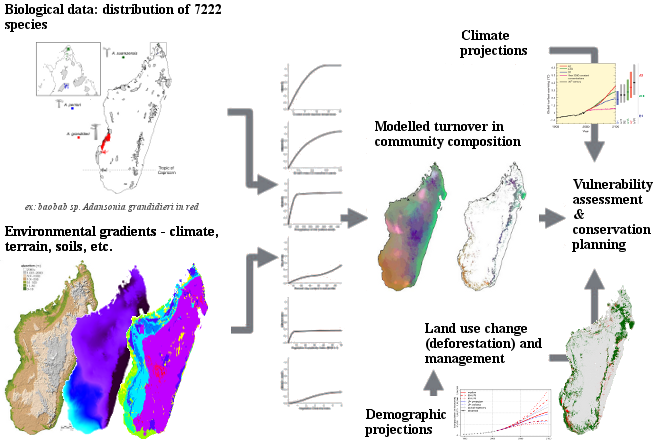
\includegraphics[width=\textwidth]{figures/Scheme} 

}

\caption{\textbf{Description schématique du projet.} Les modèles
combinent des données d'inventaires, des données environnementales et
des données démographiques pour évaluer l'impact futur des changements
climatiques et de la déforestation sur la biodiversité à Madagascar. Les
résultats sont utilisés pour une aide à la décision en aménagement du
territoire et pour définir des stratégies de conservation efficaces.}\label{fig:schema}
\end{figure}

\hypertarget{developpement-de-modeles-et-scenarios-de-la-biodiversite}{%
\subsubsection{Développement de modèles et scénarios de la
biodiversité}\label{developpement-de-modeles-et-scenarios-de-la-biodiversite}}

\hypertarget{modelisation-de-lintensite-de-la-deforestation}{%
\paragraph{Modélisation de l'intensité de la
déforestation}\label{modelisation-de-lintensite-de-la-deforestation}}

\hypertarget{modelisation-spatialisee-de-la-deforestation}{%
\paragraph{Modélisation spatialisée de la
déforestation}\label{modelisation-spatialisee-de-la-deforestation}}

\hypertarget{modelisation-de-la-niche-climatique-des-especes}{%
\paragraph{Modélisation de la niche climatique des
espèces}\label{modelisation-de-la-niche-climatique-des-especes}}

\hypertarget{modelisation-de-lassemblage-des-especes-en-communaute}{%
\paragraph{Modélisation de l'assemblage des espèces en
communauté}\label{modelisation-de-lassemblage-des-especes-en-communaute}}

\hypertarget{principaux-resultats}{%
\subsubsection{Principaux résultats}\label{principaux-resultats}}

\hypertarget{madaclim-portail-de-donnees-climatiques-et-environnementales-a-madagascar-1}{%
\paragraph{MadaClim: portail de données climatiques et environnementales
à
Madagascar}\label{madaclim-portail-de-donnees-climatiques-et-environnementales-a-madagascar-1}}

Dans le cadre du projet BioSceneMada, nous avons développé le site
internet MadaClim (\url{https://madaclim.cirad.fr}). Ce site reprend
toutes les données climatiques actuelles fournies par WorldClim ainsi
que les prédictions climatiques issues des modèles du GIEC (groupe
d'experts intergouvernemental sur l'évolution du climat) et fournies par
le CGIAR CCAFS. Les données sont recompilées (reprojetées et
rééchantillonnées à 1km) et distribuées spécifiquement pour Madagascar.
Des variables bioclimatiques supplémentaires comme l'évapotranspiration
et le nombre de mois secs ont été calculées et ajoutées aux variables
déjà disponibles. En plus des données climatiques, des données
environnementales (sol, géologie, altitude, etc.) sont également
fournies. Ce site et ces données sont particulièrement utiles pour tous
les chercheurs, gestionnaires, membres d'ONG environnementales,
ministères voulant étudier les effets du changement climatique à
Madagascar. Elles peuvent être utilisées par exemple pour calculer les
anomalies climatiques prédites par les modèles du GIECC
(Fig.~\ref{fig:anomalies}).


















\begin{figure}[H]

{\centering 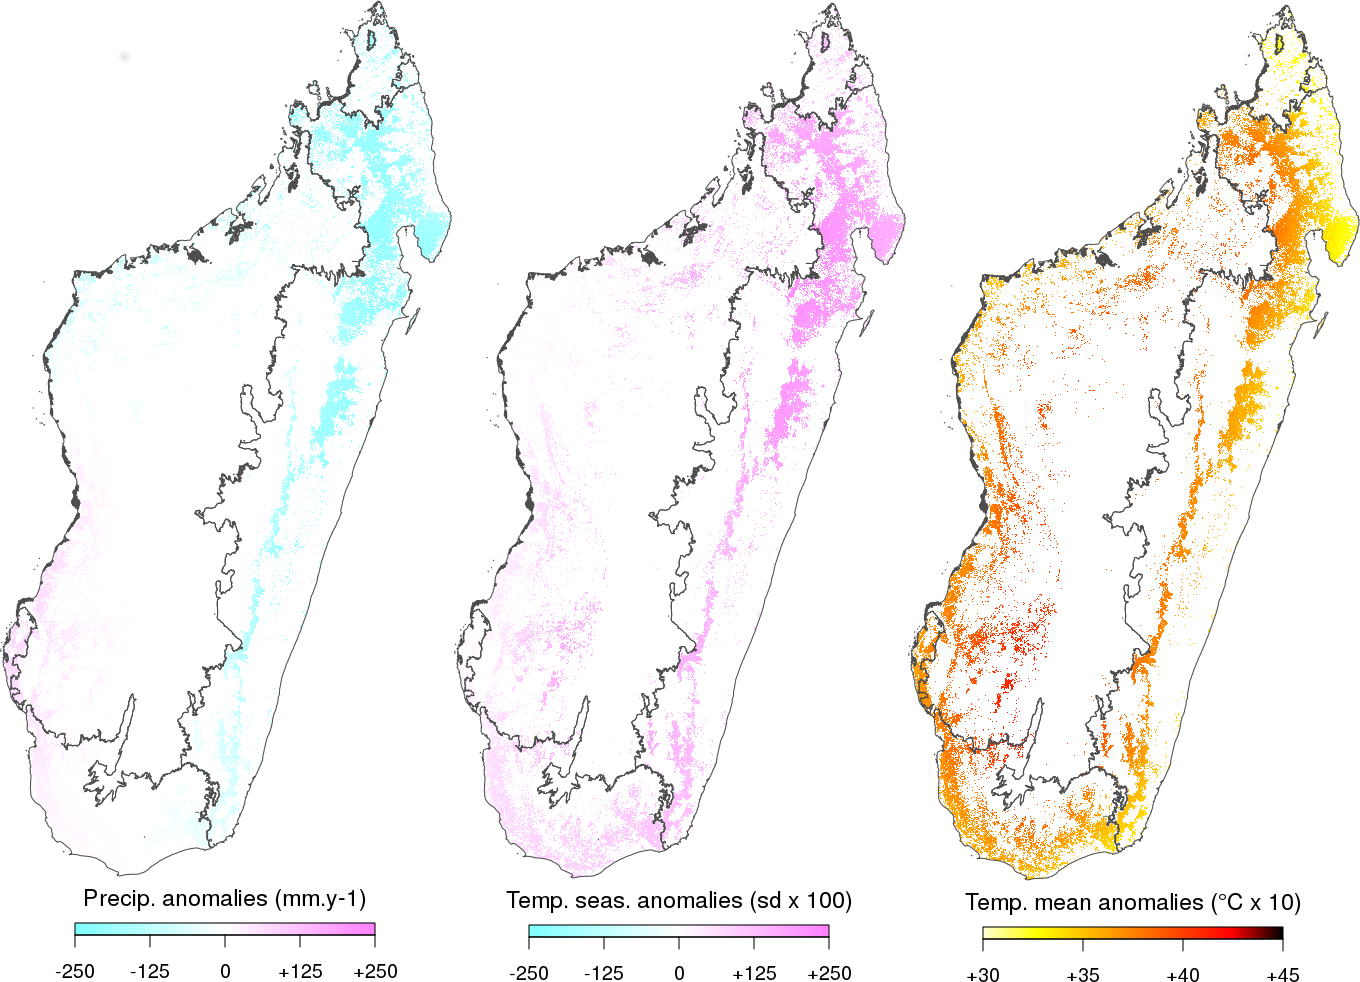
\includegraphics[width=\textwidth]{figures/Anomalies} 

}

\caption{\textbf{Anomalies climatiques prédites sur les
forêts de Madagascar entre 2010 et 2080.} Les anomalies ont été
calculées pour les précipitations annuelles (panneau de gauche), la
saisonnalité de la température (milieu) et la température moyenne
annuelle (droite) en faisant la moyenne des prédictions de sept modèles
climatiques du GIEC suivant le scénario d'émission RCP 8.5. Les
précipitations devraient diminuer, notamment sur les forêts humides de
l'est et la saisonnalité de la température ainsi que la température
moyenne annuelle devraient augmenter sur l'ensemble des forêts de
Madagascar.}\label{fig:anomalies}
\end{figure}

\hypertarget{carte-de-carbone-forestier-et-vulnerabilite-des-forets-tropicales-au-changement-climatique-a-madagascar-1}{%
\paragraph{Carte de carbone forestier et vulnérabilité des forêts
tropicales au changement climatique à
Madagascar}\label{carte-de-carbone-forestier-et-vulnerabilite-des-forets-tropicales-au-changement-climatique-a-madagascar-1}}

Dans le cadre du projet BioSceneMada, en utilisant les données
climatiques précédemment calculées (\url{https://madaclim.cirad.fr}) et
des données d'inventaires forestiers pour 1771 placettes réparties sur
l'ensemble de Madagascar, nous avons démontré qu'il existait un lien
fort entre climat et stocks de carbone forestiers. Ce lien est notamment
déterminé par les caractéristiques architecturales (hauteur notamment)
des espèces d'arbres présentes le long du gradient climatique à
Madagascar (climat --\textgreater{} assemblage d'espèces
--\textgreater{} stocks de carbone). Ainsi, les stocks de carbone sont
en moyenne beaucoup plus faibles en forêt épineuse (17 Mg.ha\(^{-1}\))
qu'en forêt humide (150 Mg.ha\(^{-1}\)). Le modèle statistique intégrant
la relation climat-stock de carbone a permis de produire une carte
précise des stocks de carbone forestier à Madagascar à une résolution de
250 m. Cette carte pourra être utilisée par les instances
gouvernementales à Madagascar ou les porteurs de projet REDD+ au niveau
régional pour le calcul des émissions de CO2 associées à la
déforestation. Cette carte ainsi que les données qui ont permis de
l'obtenir sont disponibles sur le site du projet BioSceneMada
(\url{https://bioscenemada.cirad.fr/carbonmaps}) ainsi que sur le
serveur de données Dryad (doi:
\href{http://doi.org/10.5061/dryad.9ph68}{10.5061/dryad.9ph68}).

Concernant les scénarios d'évolution de la biodiversité et des stocks de
carbone forestier, nous avons montré à l'aide de ce modèle que les
changements climatiques devraient induire des modifications fortes des
communautés forestières et en conséquence une diminution de -17\%
(7-24\%) des stocks de carbone forestier à Madagascar à l'horizon 2100
par rapport à 2010 (Fig.~\ref{fig:carbonmaps}). Ces changements seront
vraisemblablement plus forts pour la forêt humide de l'est (notamment
autour de la péninsule de Masoala-Makira) que pour les forêts sèches et
épineuses de l'ouest et du sud. En comparaison, un taux de déforestation
constant de 0.5\% par an conduirait à une perte de carbone forestier de
l'ordre de 29\% entre 2010 et 2100. L'impact potentiel des changements
climatiques sur les émissions de CO2 n'est donc pas à négliger.







\begin{figure}[H]

{\centering 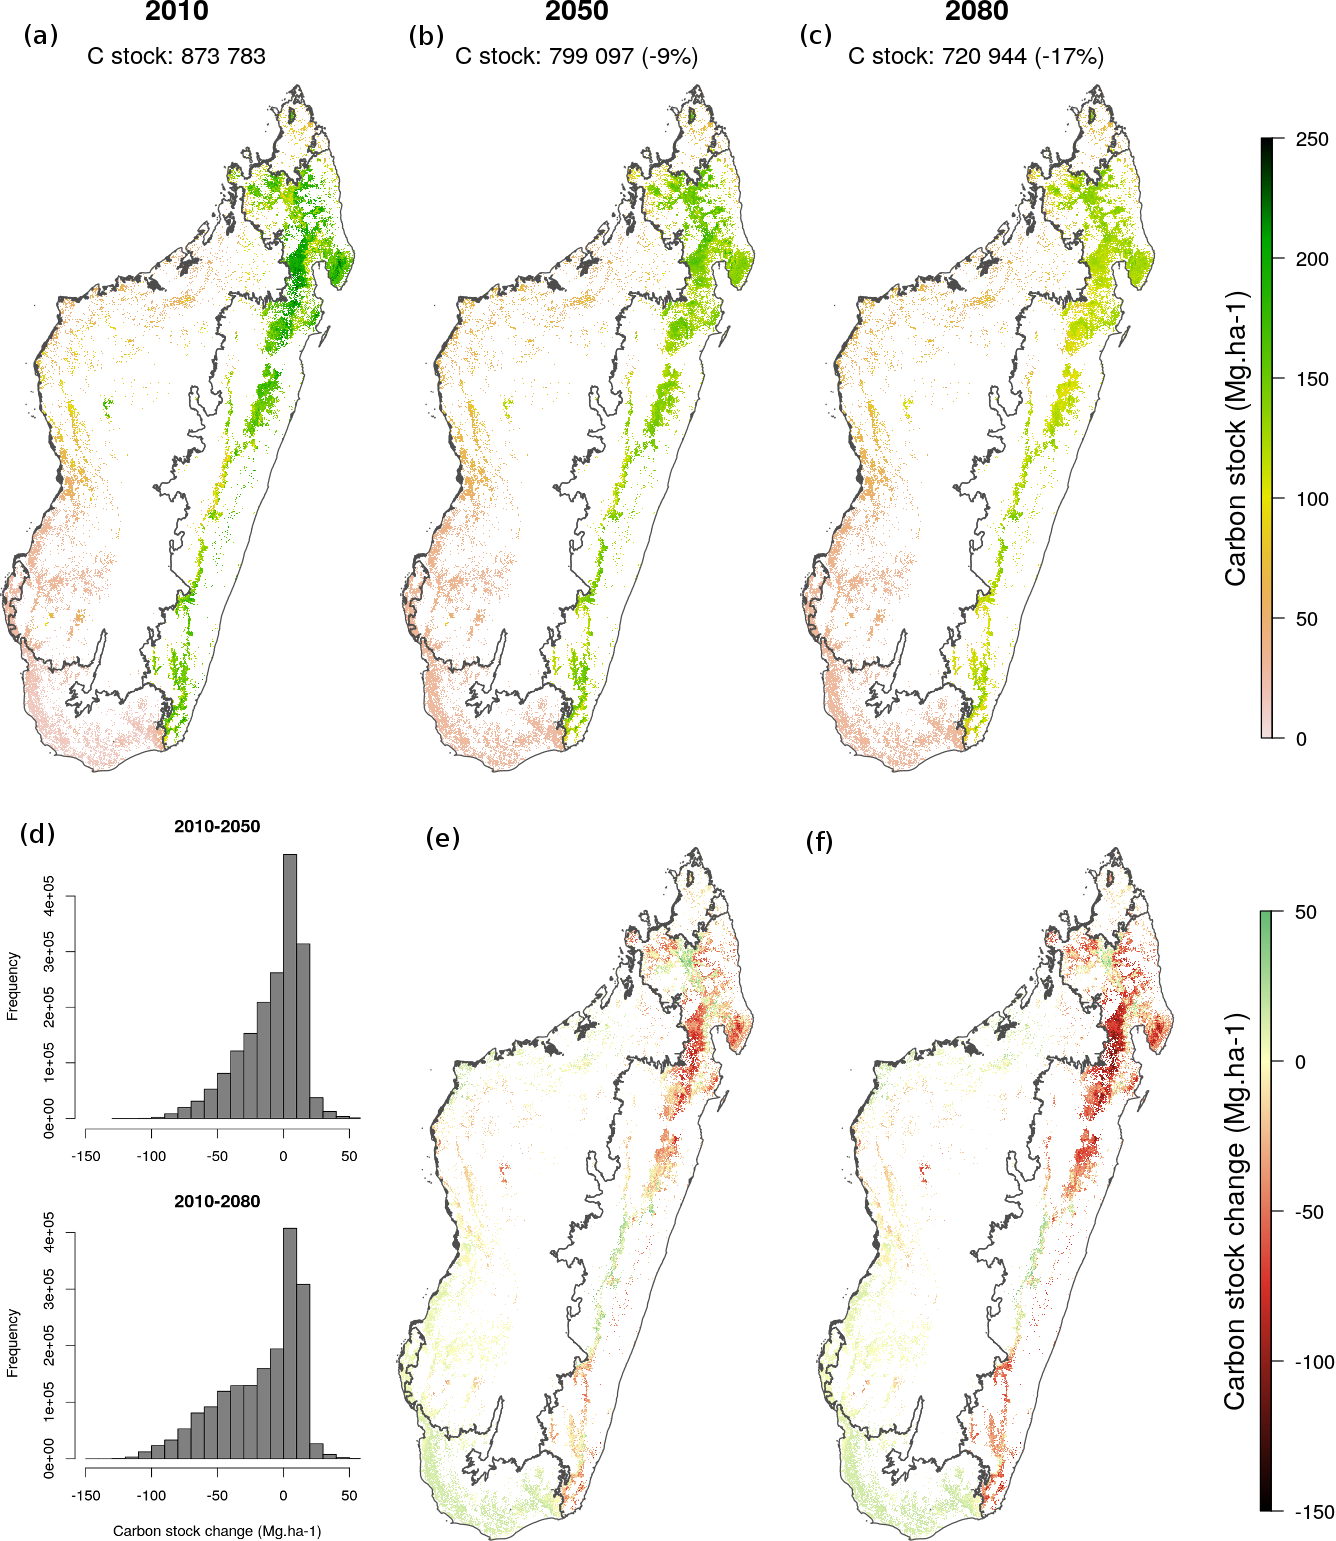
\includegraphics[width=\textwidth]{figures/carbonmaps} 

}

\caption{\textbf{Carte de carbone forestier et évolution
potentielle des stocks sous l'effet du changement climatique.} Les
changements climatiques devraient induire des modifications fortes des
communautés forestières et en conséquence une diminution des stocks de
carbone forestier (-17\% en 2100 par rapport à 2010).}\label{fig:carbonmaps}
\end{figure}

\hypertarget{base-de-donnees-de-biodiversite-a-madagascar-1}{%
\paragraph{Base de données de biodiversité à
Madagascar}\label{base-de-donnees-de-biodiversite-a-madagascar-1}}

Nous avons construit un jeu de données sur la biodiversité à Madagascar
regroupant 300~000 observations (points de présence) pour 4969 espèces.
Ces espèces sont réparties dans différents groupes taxonomiques
(Plantes, Vertébrés, Invertébrés) et sont représentatives de la
biodiversité à Madagascar (Tab. 2). Nous avons apporté une attention
particulière à la qualité des données. Toutes les données ont été
vérifiées du point de vue des coordonnées géographiques (issues de
relevés GPS) et de la taxonomie. Pour la vérification de la taxonomie,
nous nous sommes appuyés sur le package \texttt{taxize} disponible sous
le logiciel \texttt{R}. Ce travail de compilation de données de
biodiversité est sans précédent à Madagascar. Les précédentes études
scientifiques sur la biodiversité à l'échelle nationale à Madagascar
s'appuyait sur un nombre d'espèces \textless{} 2843 (Allnutt et al.
2008; Kremen et al. 2008). Plusieurs institutions ont accepté de
partager leur données de biodiversité dans le cadre du projet
BioSceneMada et ont ainsi largement contribué à la réalisation de cette
base de données. Ces données sont souvent issues d'un travail de
prospection conséquent qui s'étalent sur plusieurs dizaines d'années.

\begin{longtable}[]{@{}llrrr@{}}
\toprule
\begin{minipage}[b]{0.21\columnwidth}\raggedright
\strut
\end{minipage} & \begin{minipage}[b]{0.18\columnwidth}\raggedright
Groupe\strut
\end{minipage} & \begin{minipage}[b]{0.13\columnwidth}\raggedleft
Espèces\strut
\end{minipage} & \begin{minipage}[b]{0.11\columnwidth}\raggedleft
Genres\strut
\end{minipage} & \begin{minipage}[b]{0.14\columnwidth}\raggedleft
Obs.\strut
\end{minipage}\tabularnewline
\midrule
\endhead
\begin{minipage}[t]{0.21\columnwidth}\raggedright
\textbf{Plantes}\strut
\end{minipage} & \begin{minipage}[t]{0.18\columnwidth}\raggedright
Arbres\strut
\end{minipage} & \begin{minipage}[t]{0.13\columnwidth}\raggedleft
531\strut
\end{minipage} & \begin{minipage}[t]{0.11\columnwidth}\raggedleft
283\strut
\end{minipage} & \begin{minipage}[t]{0.14\columnwidth}\raggedleft
40178\strut
\end{minipage}\tabularnewline
\begin{minipage}[t]{0.21\columnwidth}\raggedright
\strut
\end{minipage} & \begin{minipage}[t]{0.18\columnwidth}\raggedright
Palmiers\strut
\end{minipage} & \begin{minipage}[t]{0.13\columnwidth}\raggedleft
178\strut
\end{minipage} & \begin{minipage}[t]{0.11\columnwidth}\raggedleft
16\strut
\end{minipage} & \begin{minipage}[t]{0.14\columnwidth}\raggedleft
5105\strut
\end{minipage}\tabularnewline
\begin{minipage}[t]{0.21\columnwidth}\raggedright
\strut
\end{minipage} & \begin{minipage}[t]{0.18\columnwidth}\raggedright
Fougères\strut
\end{minipage} & \begin{minipage}[t]{0.13\columnwidth}\raggedleft
317\strut
\end{minipage} & \begin{minipage}[t]{0.11\columnwidth}\raggedleft
82\strut
\end{minipage} & \begin{minipage}[t]{0.14\columnwidth}\raggedleft
1664\strut
\end{minipage}\tabularnewline
\begin{minipage}[t]{0.21\columnwidth}\raggedright
\strut
\end{minipage} & \begin{minipage}[t]{0.18\columnwidth}\raggedright
Légumineuses\strut
\end{minipage} & \begin{minipage}[t]{0.13\columnwidth}\raggedleft
724\strut
\end{minipage} & \begin{minipage}[t]{0.11\columnwidth}\raggedleft
149\strut
\end{minipage} & \begin{minipage}[t]{0.14\columnwidth}\raggedleft
30305\strut
\end{minipage}\tabularnewline
\begin{minipage}[t]{0.21\columnwidth}\raggedright
\strut
\end{minipage} & \begin{minipage}[t]{0.18\columnwidth}\raggedright
Graminées\strut
\end{minipage} & \begin{minipage}[t]{0.13\columnwidth}\raggedleft
283\strut
\end{minipage} & \begin{minipage}[t]{0.11\columnwidth}\raggedleft
113\strut
\end{minipage} & \begin{minipage}[t]{0.14\columnwidth}\raggedleft
3469\strut
\end{minipage}\tabularnewline
\begin{minipage}[t]{0.21\columnwidth}\raggedright
\strut
\end{minipage} & \begin{minipage}[t]{0.18\columnwidth}\raggedright
Autres\strut
\end{minipage} & \begin{minipage}[t]{0.13\columnwidth}\raggedleft
1229\strut
\end{minipage} & \begin{minipage}[t]{0.11\columnwidth}\raggedleft
359\strut
\end{minipage} & \begin{minipage}[t]{0.14\columnwidth}\raggedleft
34265\strut
\end{minipage}\tabularnewline
\begin{minipage}[t]{0.21\columnwidth}\raggedright
\textbf{Vertébrés}\strut
\end{minipage} & \begin{minipage}[t]{0.18\columnwidth}\raggedright
Mammifères\strut
\end{minipage} & \begin{minipage}[t]{0.13\columnwidth}\raggedleft
189\strut
\end{minipage} & \begin{minipage}[t]{0.11\columnwidth}\raggedleft
69\strut
\end{minipage} & \begin{minipage}[t]{0.14\columnwidth}\raggedleft
28316\strut
\end{minipage}\tabularnewline
\begin{minipage}[t]{0.21\columnwidth}\raggedright
\strut
\end{minipage} & \begin{minipage}[t]{0.18\columnwidth}\raggedright
Lémuriens\strut
\end{minipage} & \begin{minipage}[t]{0.13\columnwidth}\raggedleft
64\strut
\end{minipage} & \begin{minipage}[t]{0.11\columnwidth}\raggedleft
15\strut
\end{minipage} & \begin{minipage}[t]{0.14\columnwidth}\raggedleft
3136\strut
\end{minipage}\tabularnewline
\begin{minipage}[t]{0.21\columnwidth}\raggedright
\strut
\end{minipage} & \begin{minipage}[t]{0.18\columnwidth}\raggedright
Oiseaux\strut
\end{minipage} & \begin{minipage}[t]{0.13\columnwidth}\raggedleft
285\strut
\end{minipage} & \begin{minipage}[t]{0.11\columnwidth}\raggedleft
172\strut
\end{minipage} & \begin{minipage}[t]{0.14\columnwidth}\raggedleft
60895\strut
\end{minipage}\tabularnewline
\begin{minipage}[t]{0.21\columnwidth}\raggedright
\strut
\end{minipage} & \begin{minipage}[t]{0.18\columnwidth}\raggedright
Reptiles\strut
\end{minipage} & \begin{minipage}[t]{0.13\columnwidth}\raggedleft
153\strut
\end{minipage} & \begin{minipage}[t]{0.11\columnwidth}\raggedleft
41\strut
\end{minipage} & \begin{minipage}[t]{0.14\columnwidth}\raggedleft
4938\strut
\end{minipage}\tabularnewline
\begin{minipage}[t]{0.21\columnwidth}\raggedright
\strut
\end{minipage} & \begin{minipage}[t]{0.18\columnwidth}\raggedright
Amphibiens\strut
\end{minipage} & \begin{minipage}[t]{0.13\columnwidth}\raggedleft
78\strut
\end{minipage} & \begin{minipage}[t]{0.11\columnwidth}\raggedleft
21\strut
\end{minipage} & \begin{minipage}[t]{0.14\columnwidth}\raggedleft
208\strut
\end{minipage}\tabularnewline
\begin{minipage}[t]{0.21\columnwidth}\raggedright
\textbf{Invertébrés}\strut
\end{minipage} & \begin{minipage}[t]{0.18\columnwidth}\raggedright
Escargots\strut
\end{minipage} & \begin{minipage}[t]{0.13\columnwidth}\raggedleft
537\strut
\end{minipage} & \begin{minipage}[t]{0.11\columnwidth}\raggedleft
113\strut
\end{minipage} & \begin{minipage}[t]{0.14\columnwidth}\raggedleft
1635\strut
\end{minipage}\tabularnewline
\begin{minipage}[t]{0.21\columnwidth}\raggedright
\strut
\end{minipage} & \begin{minipage}[t]{0.18\columnwidth}\raggedright
Fourmis\strut
\end{minipage} & \begin{minipage}[t]{0.13\columnwidth}\raggedleft
379\strut
\end{minipage} & \begin{minipage}[t]{0.11\columnwidth}\raggedleft
46\strut
\end{minipage} & \begin{minipage}[t]{0.14\columnwidth}\raggedleft
70012\strut
\end{minipage}\tabularnewline
\begin{minipage}[t]{0.21\columnwidth}\raggedright
\strut
\end{minipage} & \begin{minipage}[t]{0.18\columnwidth}\raggedright
Papillons\strut
\end{minipage} & \begin{minipage}[t]{0.13\columnwidth}\raggedleft
262\strut
\end{minipage} & \begin{minipage}[t]{0.11\columnwidth}\raggedleft
82\strut
\end{minipage} & \begin{minipage}[t]{0.14\columnwidth}\raggedleft
16396\strut
\end{minipage}\tabularnewline
\begin{minipage}[t]{0.21\columnwidth}\raggedright
\strut
\end{minipage} & \begin{minipage}[t]{0.18\columnwidth}\raggedright
Autres\strut
\end{minipage} & \begin{minipage}[t]{0.13\columnwidth}\raggedleft
355\strut
\end{minipage} & \begin{minipage}[t]{0.11\columnwidth}\raggedleft
203\strut
\end{minipage} & \begin{minipage}[t]{0.14\columnwidth}\raggedleft
6202\strut
\end{minipage}\tabularnewline
\begin{minipage}[t]{0.21\columnwidth}\raggedright
\textbf{TOTAL=}\strut
\end{minipage} & \begin{minipage}[t]{0.18\columnwidth}\raggedright
\strut
\end{minipage} & \begin{minipage}[t]{0.13\columnwidth}\raggedleft
\textbf{4969}\strut
\end{minipage} & \begin{minipage}[t]{0.11\columnwidth}\raggedleft
1749\strut
\end{minipage} & \begin{minipage}[t]{0.14\columnwidth}\raggedleft
\textbf{303588}\strut
\end{minipage}\tabularnewline
\bottomrule
\end{longtable}

Table 2: \textbf{Bases de données sur la biodiversité de Madagascar.} La
base de données incluent des points de présence pour 4969 espèces
réparties dans différents groupes taxonomiques. Ces espèces sont
représentatives de la biodiversité à Madagascar.

\hypertarget{atlas-de-la-biodiversite-a-madagascar-et-de-sa-vulnerabilite-au-changement-climatique-1}{%
\paragraph{Atlas de la biodiversité à Madagascar et de sa vulnérabilité
au changement
climatique}\label{atlas-de-la-biodiversite-a-madagascar-et-de-sa-vulnerabilite-au-changement-climatique-1}}

Nous avons développé un script permettant de modéliser la niche
climatique des espèces à partir de modèles d'ensemble (Vieilledent et
al. 2013; Araujo and New 2007). Ce script utilise le package
\texttt{biomod2} sous \texttt{R}. A partir de variables
environnementales, incluant des variables climatiques (température
moyenne annuelle, saisonnalité de la température, précipitations
annuelles, déficit en eau, nombre de mois secs) et des variables
physiques (radiation solaire, géologie) disponibles sur le site
\href{https://madaclim.cirad.fr}{MadaClim}, il permet de prédire la
probabilité de présence ainsi que l'aire de distribution présente et
future des espèces à Madagascar. Les prédictions sont issues de
plusieurs modèles statistiques (Maxent, GLM, GAM et Random Forest).
L'approche par modèles d'ensemble permet de moyenner les prédictions
faites par plusieurs modèles statistiques afin d'évaluer l'incertitude
des prédictions et d'augmenter la robustesse de l'aire de distribution.
Le script a été développé au cours du stage de Master II de Mario
Muniz-Tagliari. L'idée est de pouvoir utiliser ce script et modéliser
l'aire de distribution présente et future de l'ensemble des espèces
constituant le jeu de données sur la biodiversité à Madagascar (4969
espèces).

Le script a été optimisé. Il peut être parrallélisé, c'est-à-dire envoyé
sur les différents processeurs d'un serveur afin d'accélérer les
calculs. Il permet également de créer un document pdf dynamique,
réactualisable très facilement, où les photos, textes, figures et
tableaux sont agencés de manière automatique pour chaque espèce
(Fig.~\ref{fig:atlas}). La dernière version du script est disponible sur
GitHub: \url{https://github.com/ghislainv/atlas}. Ce répertoire est
privé pour le moment mais accessible avec le couple d'identifiants
suivant sur la plateforme GitHub: \texttt{gvguest}/\texttt{gvguest!1}.
L'objectif est d'obtenir au final un atlas de la biodiversité à
Madagascar incluant (i) les points de présence des espèces, (ii) leur
aire de distribution actuelle, (iii) la distribution future potentielle
des espèces sous l'effet du changement climatique et une estimation de
leur vulnérabilité au changement climatique.

Un prototype de cet atlas a été réalisé pour les 7 espèces de baobab
présentes à Madagascar. Le prototype de l'atlas est disponible
\href{https://bioscenemada.cirad.fr/FileTransfer/atlas.pdf}{ici}.













\begin{figure}[H]

{\centering 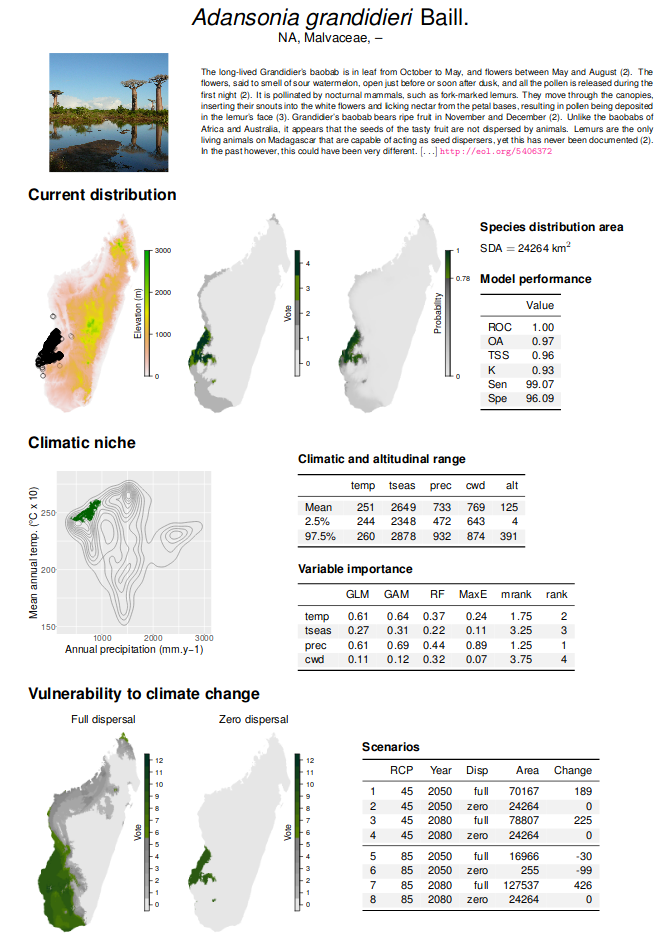
\includegraphics[width=0.8\linewidth]{figures/atlas} 

}

\caption{\textbf{Extrait de l'atlas de la biodiversité à
Madagascar et de sa vulnérabilité au changement climatique pour l'espèce
\emph{Adansonia grandidieri}.} Une fiche est dynamiquement créée à parti
du nom taxonomique de l'espèce et de ses points de présence en utilisant
un script \texttt{R}. Photo et texte sont extraits automatiquement du
site \emph{Encyclopedia Of Life} (\url{http://eol.org}). Un ensemble de
modèles statistiques est utilisé pour prédire la niche climatique et
l'aire de distribution actuelle de l'espèce. Ce modèle d'ensemble est
ensuite utilisé pour prédire la vulnérabilité de l'espèce au changement
climatique en intégrant les prédictions climatiques du GIECC suivant
deux scénarios, RCP 8.5 et 4.5.}\label{fig:atlas}
\end{figure}

\hypertarget{cartes-de-biodiversite-et-des-communautes-despeces-a-madagascar-1}{%
\paragraph{Cartes de biodiversité et des communautés d'espèces à
Madagascar}\label{cartes-de-biodiversite-et-des-communautes-despeces-a-madagascar-1}}

Lorsque l'on parle de carte de biodiversité à l'échelle nationale,
l'objectif n'est pas uniquement d'obtenir des informations sur la
localisation des ``hotspots'' ou points-chauds de la biodiversité (les
sites ayant une diversité spécifique élevée), ce que l'on appelle la
diversité \(\alpha\). Il est en effet surtout intéressant de considérer
la diversité \(\beta\), c'est-à-dire les communautés ou assemblages
d'espèces et comment les assemblages d'espèces changent spatialement
(``species turnover''), selon des gradients environnementaux
(d'altitude, de climat, etc.). De telles cartes n'existent pas
actuellement à l'échelle nationale pour Madagascar. Seules des cartes de
végétation sont disponibles pour lesquelles la classification s'appuie
sur la définition de grands biomes (\url{http://www.vegmad.org}) et non
sur des relevés à l'échelle de l'espèce, à la fois pour la faune et la
flore.

En utilisant des modèles de communautés (Ferrier et al. 2007), nous
avons cherché à identifier les facteurs environnementaux déterminants
les assemblages d'espèces. Ces facteurs peuvent être climatiques ou
associés à des barrières géographiques comme les bassins versants ou les
rivières (Pearson and Raxworthy 2009). Il ainsi été montré que la
distribution des espèces de lémuriens à Madagascar était fortement liée
aux bassins versants (Wilmé, Goodman, and Ganzhorn 2006; Mercier and
Wilmé 2013). Les modèles de communautés que nous avons utilisés, appelés
GDM (Generalized Dissimilarity Models), modélisent les changements
d'espèces au sein de la communauté en fonction des gradients
environnementaux en s'appuyant sur des indices de dissimilarités entre
sites (Ferrier et al. 2007). En appliquant ce modèle à nos données de
présence d'espèces à Madagascar, nous avons obtenu une première carte de
la biodiversité \(\beta\) à Madagascar (Fig.~\ref{fig:GDM}). Mais le
pourcentage de déviance expliquée par ce modèle est faible
(\textless{}10\%).









\begin{figure}[H]

{\centering 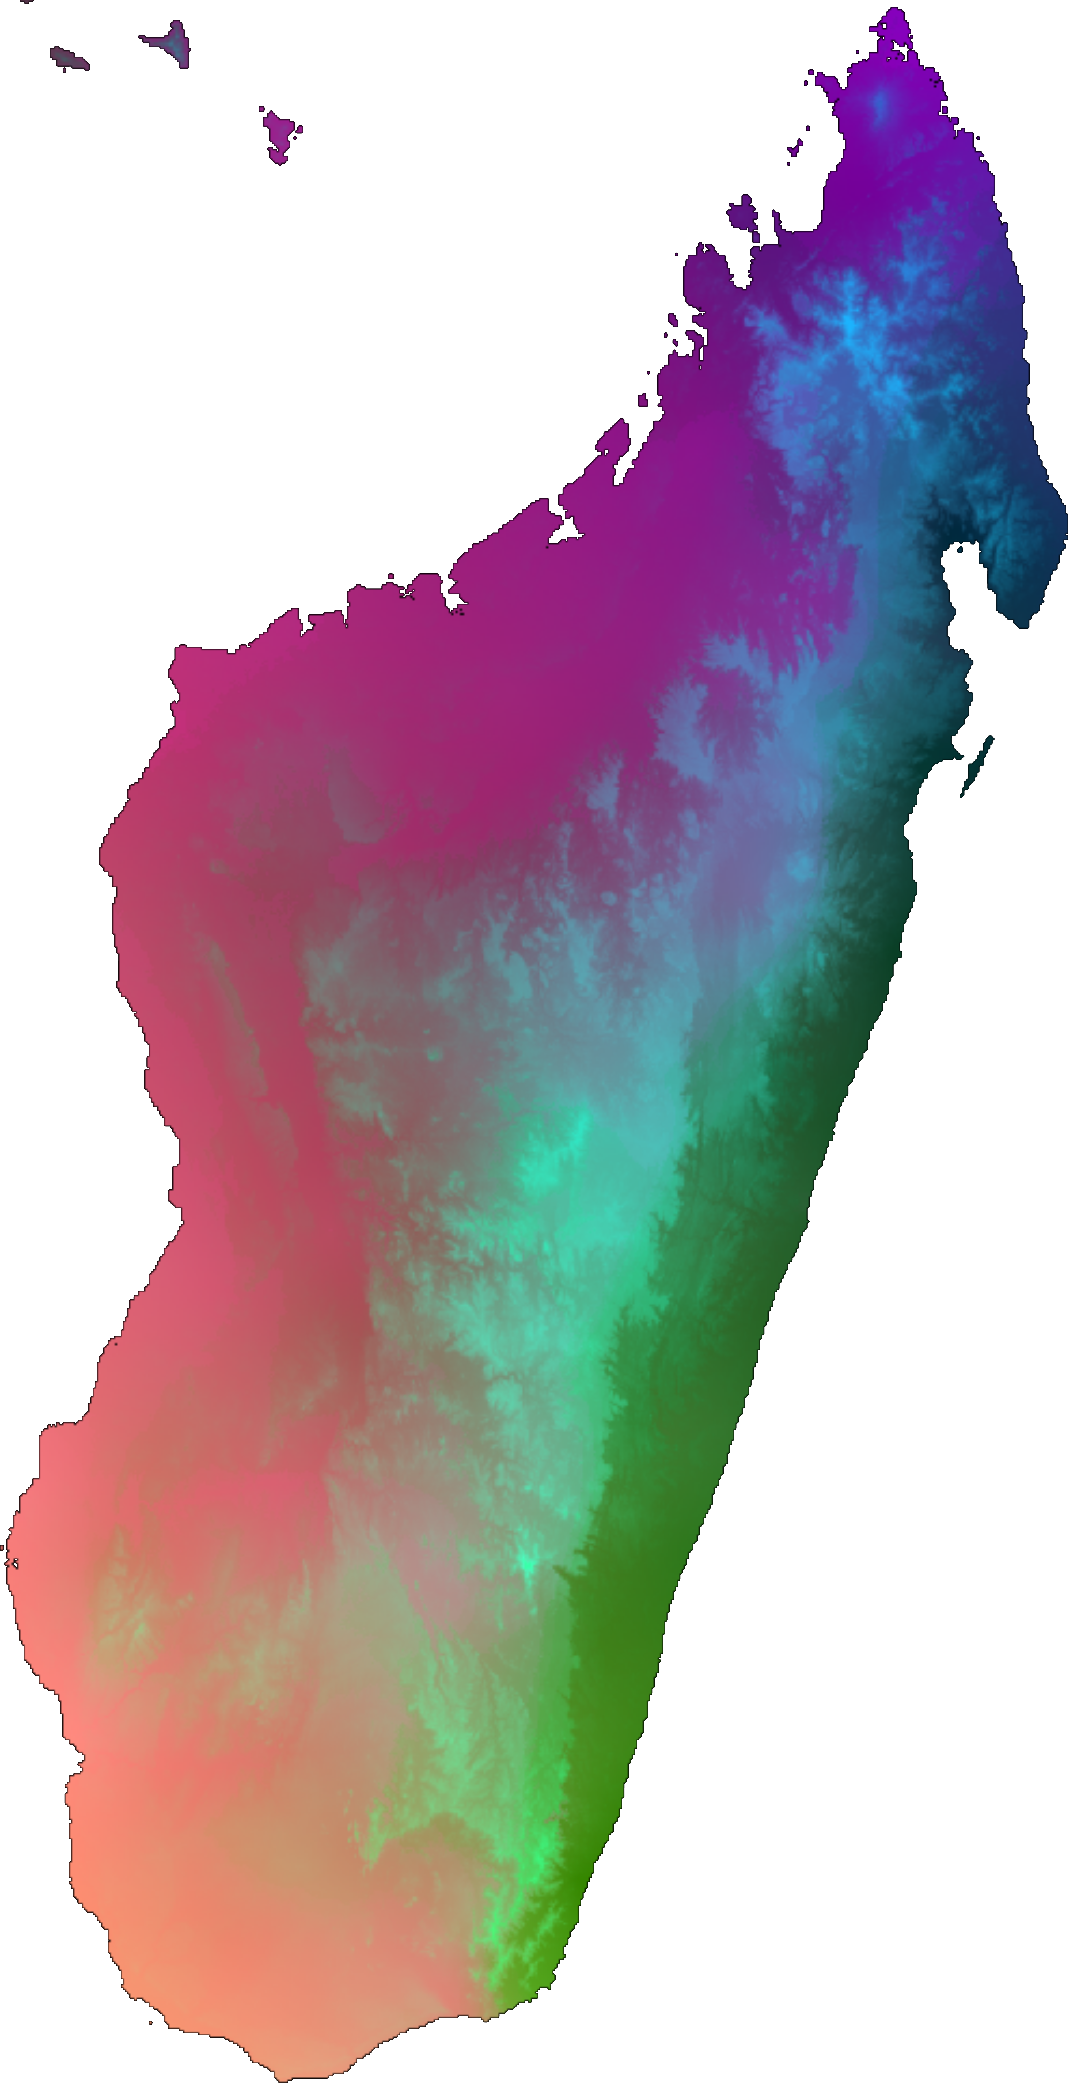
\includegraphics[width=8cm]{figures/GDM_map} 

}

\caption{\textbf{Carte de biodiversité \(\beta\) pour Madagascar.}
Les couleurs indiquent les changements d'assemblage d'espèces
spatialement: les sites aux couleurs proches présentent des assemblages
d'espèces proches. Deux gradients sont largements visibles sur cette
carte: un gradient est-ouest lié à la topographie (chaîne de montagne
nord-sud) et aux précipitations ainsi qu'un un gradient nord-sud associé
à la latitude et à la saisonnalité.}\label{fig:GDM}
\end{figure}

En applicant ce même modèle à chaque groupe taxonomique, nous avons
trouvé que (i) le pourcentage de variance expliquée par le modèle était
généralement beaucoup plus élevé (entre 11\% et 88\%, Tab.~3) et que
(ii) les facteurs explicants l'assemblage des communautés d'espèces
variaient d'un groupe taxonomique à l'autre, le climat n'étant pas
toujours le facteur le plus important (Tab.~3). Par exemple, nous avons
confirmé les résultats obtenus par Wilmé, Goodman, and Ganzhorn (2006)
pour les espèces de lémuriens. Pour ce groupe, ce sont les bassins
versants qui expliquent en majorité l'assemblage des espèces (84\% de
déviance expliquée). Cela pourrait notamment s'expliquer par la
difficulté qu'on les lémuriens à traverser les cours d'eau. A contrario,
le climat explique une grande partie des assemblages d'espèces de
reptiles et d'amphibiens, espèces poïkilothermes (animaux ayant une
température corporelle qui varie avec celle de leur milieu) et des
espèces de mammifères autres que les lémuriens. Pour d'autres groupes,
comme les espèces d'arbres, les facteurs climatiques et les bassins
versants semblent expliquer à part égale les assemblages d'espèces.

Ainsi, on voit qu'il est difficile d'établir une carte des communautés
d'espèces végétales et animales à Madagascar, les facteurs explicatifs
de la distribution des communautés changeant d'un groupe à l'autre. Nous
montrons également que lorsque l'on utilise des modèles de communautés
construits à partir de GDM, basés sur indices de dissimilarités
combinant toutes les espèces, il y a un risque d'obtenir un modèle très
peu explicatif, alors que des modèles à l'échelle du groupe taxonomique
sont bien meilleurs. Il serait ainsi nécessaire d'envisager (i) de
croiser les cartes de biodiversité obtenues par groupe taxonomique, ou
bien (ii) de travailler plutôt avec des modèles de distribution à
l'échelle de l'espèce, ou encore (iii) d'utiliser d'autres types de
modèles comme les ``modèles joints'' (Warton et al. 2015), permettant de
combiner des processus à l'échelle de l'espèce et des processus à
l'échelle de la communauté.

\begin{longtable}[]{@{}lrrrr@{}}
\toprule
\begin{minipage}[b]{0.30\columnwidth}\raggedright
Groupes\strut
\end{minipage} & \begin{minipage}[b]{0.08\columnwidth}\raggedleft
Clim\strut
\end{minipage} & \begin{minipage}[b]{0.06\columnwidth}\raggedleft
WS\strut
\end{minipage} & \begin{minipage}[b]{0.08\columnwidth}\raggedleft
C+WS\strut
\end{minipage} & \begin{minipage}[b]{0.08\columnwidth}\raggedleft
Full\strut
\end{minipage}\tabularnewline
\midrule
\endhead
\begin{minipage}[t]{0.30\columnwidth}\raggedright
\textbf{Plantes}\strut
\end{minipage} & \begin{minipage}[t]{0.08\columnwidth}\raggedleft
\strut
\end{minipage} & \begin{minipage}[t]{0.06\columnwidth}\raggedleft
\strut
\end{minipage} & \begin{minipage}[t]{0.08\columnwidth}\raggedleft
\strut
\end{minipage} & \begin{minipage}[t]{0.08\columnwidth}\raggedleft
\strut
\end{minipage}\tabularnewline
\begin{minipage}[t]{0.30\columnwidth}\raggedright
Arbres\strut
\end{minipage} & \begin{minipage}[t]{0.08\columnwidth}\raggedleft
30\strut
\end{minipage} & \begin{minipage}[t]{0.06\columnwidth}\raggedleft
28\strut
\end{minipage} & \begin{minipage}[t]{0.08\columnwidth}\raggedleft
43\strut
\end{minipage} & \begin{minipage}[t]{0.08\columnwidth}\raggedleft
44\strut
\end{minipage}\tabularnewline
\begin{minipage}[t]{0.30\columnwidth}\raggedright
Tous\strut
\end{minipage} & \begin{minipage}[t]{0.08\columnwidth}\raggedleft
24\strut
\end{minipage} & \begin{minipage}[t]{0.06\columnwidth}\raggedleft
16\strut
\end{minipage} & \begin{minipage}[t]{0.08\columnwidth}\raggedleft
31\strut
\end{minipage} & \begin{minipage}[t]{0.08\columnwidth}\raggedleft
32\strut
\end{minipage}\tabularnewline
\begin{minipage}[t]{0.30\columnwidth}\raggedright
\textbf{Animauxs}\strut
\end{minipage} & \begin{minipage}[t]{0.08\columnwidth}\raggedleft
\strut
\end{minipage} & \begin{minipage}[t]{0.06\columnwidth}\raggedleft
\strut
\end{minipage} & \begin{minipage}[t]{0.08\columnwidth}\raggedleft
\strut
\end{minipage} & \begin{minipage}[t]{0.08\columnwidth}\raggedleft
\strut
\end{minipage}\tabularnewline
\begin{minipage}[t]{0.30\columnwidth}\raggedright
Lémuriens\strut
\end{minipage} & \begin{minipage}[t]{0.08\columnwidth}\raggedleft
56\strut
\end{minipage} & \begin{minipage}[t]{0.06\columnwidth}\raggedleft
84\strut
\end{minipage} & \begin{minipage}[t]{0.08\columnwidth}\raggedleft
87\strut
\end{minipage} & \begin{minipage}[t]{0.08\columnwidth}\raggedleft
88\strut
\end{minipage}\tabularnewline
\begin{minipage}[t]{0.30\columnwidth}\raggedright
Autres mammifères\strut
\end{minipage} & \begin{minipage}[t]{0.08\columnwidth}\raggedleft
63\strut
\end{minipage} & \begin{minipage}[t]{0.06\columnwidth}\raggedleft
30\strut
\end{minipage} & \begin{minipage}[t]{0.08\columnwidth}\raggedleft
64\strut
\end{minipage} & \begin{minipage}[t]{0.08\columnwidth}\raggedleft
65\strut
\end{minipage}\tabularnewline
\begin{minipage}[t]{0.30\columnwidth}\raggedright
Oiseaux\strut
\end{minipage} & \begin{minipage}[t]{0.08\columnwidth}\raggedleft
8\strut
\end{minipage} & \begin{minipage}[t]{0.06\columnwidth}\raggedleft
3\strut
\end{minipage} & \begin{minipage}[t]{0.08\columnwidth}\raggedleft
9\strut
\end{minipage} & \begin{minipage}[t]{0.08\columnwidth}\raggedleft
11\strut
\end{minipage}\tabularnewline
\begin{minipage}[t]{0.30\columnwidth}\raggedright
Reptiles et Amphibiens\strut
\end{minipage} & \begin{minipage}[t]{0.08\columnwidth}\raggedleft
34\strut
\end{minipage} & \begin{minipage}[t]{0.06\columnwidth}\raggedleft
33\strut
\end{minipage} & \begin{minipage}[t]{0.08\columnwidth}\raggedleft
40\strut
\end{minipage} & \begin{minipage}[t]{0.08\columnwidth}\raggedleft
40\strut
\end{minipage}\tabularnewline
\begin{minipage}[t]{0.30\columnwidth}\raggedright
Invertébrés\strut
\end{minipage} & \begin{minipage}[t]{0.08\columnwidth}\raggedleft
9\strut
\end{minipage} & \begin{minipage}[t]{0.06\columnwidth}\raggedleft
3\strut
\end{minipage} & \begin{minipage}[t]{0.08\columnwidth}\raggedleft
9\strut
\end{minipage} & \begin{minipage}[t]{0.08\columnwidth}\raggedleft
11\strut
\end{minipage}\tabularnewline
\begin{minipage}[t]{0.30\columnwidth}\raggedright
Tous\strut
\end{minipage} & \begin{minipage}[t]{0.08\columnwidth}\raggedleft
6\strut
\end{minipage} & \begin{minipage}[t]{0.06\columnwidth}\raggedleft
2\strut
\end{minipage} & \begin{minipage}[t]{0.08\columnwidth}\raggedleft
6\strut
\end{minipage} & \begin{minipage}[t]{0.08\columnwidth}\raggedleft
9\strut
\end{minipage}\tabularnewline
\bottomrule
\end{longtable}

Table 3: \textbf{Facteurs explicants l'assemblage des espèces par groupe
taxonomique.} Le tableau indique le pourcentage de déviance expliquée
par chacun des modèles. Les modèles Clim n'incluent que des variables
climatiques, les modèles WS n'incluent que les bassins versants (WS pour
``watershed'') et les modèles C+WS incluent les deux types de facteurs.
Le modèle Full inclue en plus des corrélations spatiales.

\hypertarget{soixante-ans-1953-2014-detude-de-la-deforestation-et-de-la-fragmentation-forestiere-a-madagascar-1}{%
\paragraph{Soixante ans (1953-2014) d'étude de la déforestation et de la
fragmentation forestière à
Madagascar}\label{soixante-ans-1953-2014-detude-de-la-deforestation-et-de-la-fragmentation-forestiere-a-madagascar-1}}

Nous avons obtenu de nouvelles cartes d'évolution de la couverture
forestière à Madagascar sur la période 2000-2014 (Fig.~\ref{fig:fcc}).
Ces cartes sont sans nuages et disponibles à 30 m de résolution. Elles
viennent compléter les cartes de G. J. Harper et al. (2007) disponibles
pour les années 1953, 1973 et 1990. Ainsi, nous avons pu étudier
l'évolution du couvert forestier et de la fragmentation de la forêt à
l'échelle nationale sur une période de 60 ans. Nous montrons que le
couvert forestier a diminué de 44\% sur la période 1953-2014 (37\% si
l'on considère la période 1973-2014). Les forêts naturelles couvrent 8.9
Mha en 2014 (15\% du territoire national) et incluent 4.4 Mha (50\%) de
forêt humide, 2.6 Mha (29\%) de forêt sèche, 1.7 Mha de forêt épineuse
(19\%) et environ 177,000 ha (2\%) de mangrove. Depuis 2005, les
surfaces déforestées annuellement ont augmenté à Madagascar pour
atteindre 100,000 ha/an sur la période 2010-2014 (correspondant à un
taux de déforestation de 1.1 \%/an). Aujourd'hui, environ 50\% de la
forêt est située à moins de 100 m de la lisière et est donc exposée aux
perturbations. Les cartes de couvert forestier sont disponibles sur le
site du projet BioSceneMada:
\url{https://bioscenemada.cirad.fr/forestmaps}. Elles servent de base au
travail de modélisation du processus de déforestation.













\begin{figure}[H]

{\centering 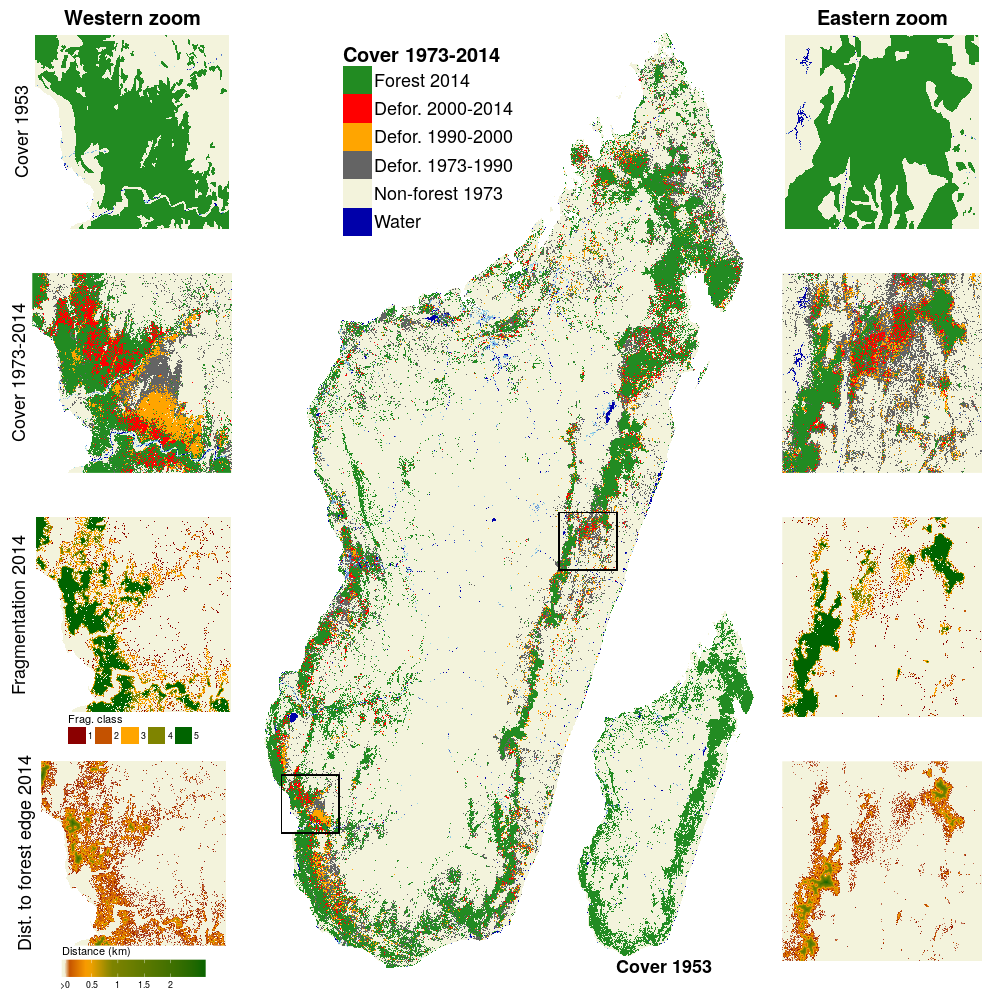
\includegraphics[width=\textwidth]{figures/fig_fcc} 

}

\caption{\textbf{Evolution du couvert forestier à Madagascar sur 60
ans de 1953 à 2014.} Les changements de couverture forestière de 1973 à
2014 sont présentés sur la figure principale. Le couvert forestier en
1953 est présenté dans l'encart en bas à droite. Deux séries de zooms
sur la forêt sèche de l'ouest (à gauche) et de la forêt humide de l'est
(à droite) presentent une vue plus détaillée de (du haut vers le bas):
la couverture forestière en 1953, les changements de couverture
forestière de 1973 à 2014, la fragmentation de la forêt en 2014 et la
distance à la lisière de la forêt en 2014. Les données sur les plans
d'eau et leur saisonnalité (bleu foncé pour permanent, bleu clair pour
saisonnié) sont issues de l'article de (Pekel et al. 2016).}\label{fig:fcc}
\end{figure}

\hypertarget{retour-sur-les-facteurs-de-deforestation-la-pauvrete-nest-pas-lunique-responsable-de-la-deforestation-a-madagascar.-1}{%
\paragraph{Retour sur les facteurs de déforestation: la pauvreté n'est
pas l'unique responsable de la déforestation à
Madagascar.}\label{retour-sur-les-facteurs-de-deforestation-la-pauvrete-nest-pas-lunique-responsable-de-la-deforestation-a-madagascar.-1}}

Afin de valider les cartes de déforestation historique obtenues sur la
période 2000-2014 et d'identifier plus précisément les facteurs de
déforestation, nous avons effectué une mission de terrain dans le
Menabe, à l'ouest de Madagascar, en forêt sèche. Nous nous sommes
concentrés sur deux zones identifiées comme ``hot-spot'' de
déforestation, autour des Parcs Nationaux de Menabe-Antimena et
Kirindy‐Mité. Nous avons effectué des observations de terrain ainsi que
des enquêtes auprès des populations et de l'administration locale afin
d'identifier les causes de la déforestation. Nous avons conclu que les
causes directes de la déforestation dans la région sont l'agriculture
sur brulis pour la culture de rente comme le maïs ou l'arachide et le
paturage des zébus (Fig.~\ref{fig:causes}). Le maïs et l'arachide sont
principalement exportés sur les marchés internationaux, notamment vers
les îles de l'Océan Indien et en Chine. Ces activités sont favorisées
par un marché global non régulé, une forte corruption et une
non-application des lois environnementales à Madagascar. Dans
l'hypothèse d'un scénario ``business-as-usual'', si aucune solution
n'est trouvée pour lutter efficacement contre la déforestation, le
couvert forestier pourrait diminuer de plus de 50\% sur la période
2010-2050 dans les deux zones d'étude.

















\begin{figure}[H]

{\centering 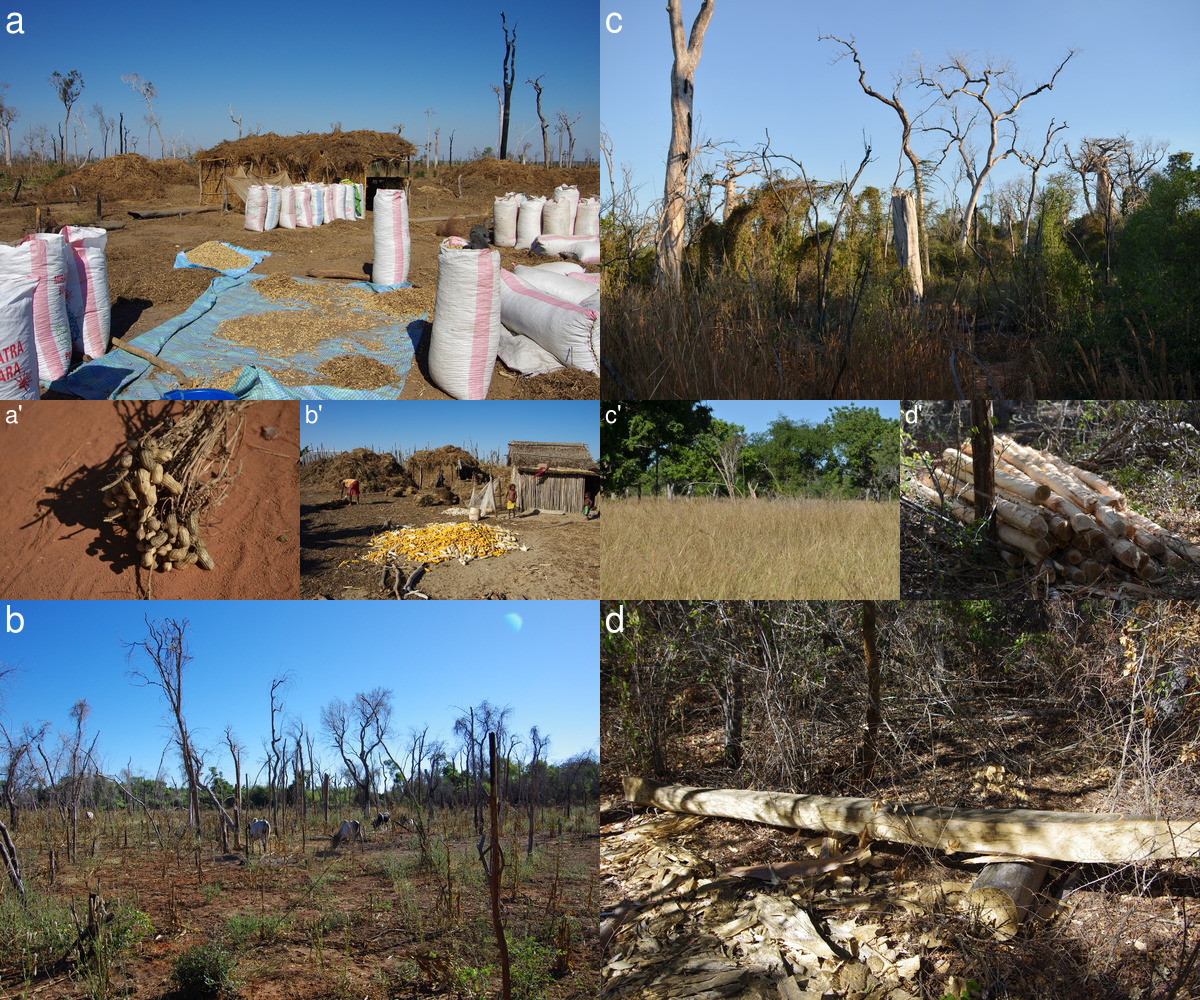
\includegraphics[width=\textwidth]{figures/causes} 

}

\caption{\textbf{Principales causes de la déforestation dans le
Menabe centrale.} \textbf{a-a'}: Agriculture sur brulis
(\emph{``hatsake''}) pour la culture d'arachide. \textbf{b-b'}:
Agriculture sur brulis pour la culture de maïs. \textbf{c-c'}: Cyclone
suivi de feux incontrolés d'origine anthropique. \textbf{d-d'}:
Exploitation illégale de bois.}\label{fig:causes}
\end{figure}

\hypertarget{logiciel-python-deforestprob-pour-le-calcul-de-la-probabilite-spatiale-de-deforestation}{%
\paragraph{\texorpdfstring{Logiciel Python \texttt{deforestprob} pour le
calcul de la probabilité spatiale de
déforestation}{Logiciel Python deforestprob pour le calcul de la probabilité spatiale de déforestation}}\label{logiciel-python-deforestprob-pour-le-calcul-de-la-probabilite-spatiale-de-deforestation}}

Un module Python a été développé afin de pouvoir estimer rapidement la
probabilité spatiale de déforestation sur de grandes échelles spatiales
(nationales ou continentales) avec une résolution fine (ex. 30 ou 10 m)
et de prédire quelles seront les zones à risques de déforestation et les
zones potentielles de refuge de la biodiversité dans le futur. Le modèle
portant sur la localisation de la déforestation permet de prédire la
probabilité spatiale de déforestation en fonction de variables
environnementales décrivant l'accessibilité de la forêt (distance aux
routes, villages et rivières, distance à la lisière de la forêt,
topographie), son statut de protection (appartenance au réseau d'aires
naturelles protégées) et son historique (distance à la déforestation
passée). Le module Python est disponible sur le serveur Github:
\url{https://github.com/ghislainv/deforestprob}.

Nous avons utilisé ce module pour estimer la probabilité spatiale de
déforestation à l'échelle nationale à Madagascar, à une résolution fine
de 30 m et pour la couverture forestière de l'année 2010
(Fig.~\ref{fig:pred}). Cette démarche a fait l'objet d'un tutoriel où
chacune des étape de modélisation est indiquée pas à pas. Cet tutoriel,
disponible sous forme d'un notebook Jupyter est disponible à l'adresse
suivante: \url{https://ghislainv.github.io/deforestprob}. Le tutoriel
pourra notamment être utilisé pendant les ateliers de renforcement de
capacité dans les deux prochaines années à venir.







\begin{figure}[H]

{\centering 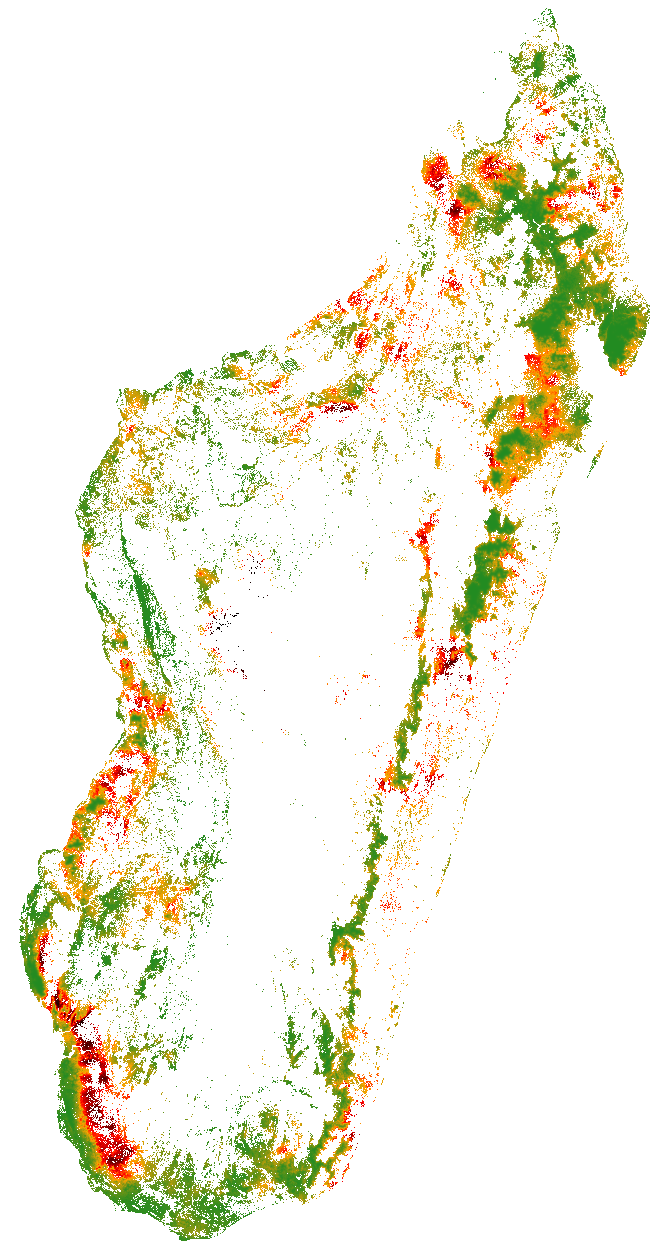
\includegraphics[width=10cm]{figures/pred_binomial_iCAR} 

}

\caption{\textbf{Probabilité de déforestation pour les forêts de
Madagascar.} Couvert forestier de l'année 2010 (Vieilledent et al.
2017). La probabilité de déforestation est faible (vert) dans les zones
reculées et au sein des aires protégées et augmente (rouge puis noir)
avec la proximité des villes et des routes.}\label{fig:pred}
\end{figure}

\hypertarget{cartes-du-couvert-forestier-futur-a-madagascar-1}{%
\paragraph{Cartes du couvert forestier futur à
Madagascar}\label{cartes-du-couvert-forestier-futur-a-madagascar-1}}

A partir de la carte de probabilité de déforestation de 2010, en
considérant une déforestation moyenne annuelle de 100~000 ha/an à
l'échelle nationale sur la période 2010-2050, nous avons pu prédire les
zones susceptibles d'être déforestées sur la période 2010-2050 et la
couverture forestière probable à Madagascar en 2050
(Fig.~\ref{fig:fc2050}). Pour cela, nous calculons la surface forestière
déforestée sur une période de 40 ans entre 2010 et 2050 (4 Mha) et nous
attribuons la classe ``non-forêt'' aux pixels ayant la plus forte
probabilité de déforestation jusqu'à obtenir une surface de 4 Mha. Les
projections montrent une concentration des forêts dans les zones peu
accessibles et situées en altitude dans le futur, notamment autour de la
péninsule de Mosoala-Makira et dans le Corridor Ankeniheny-Zahamena
(Fig. 8). Les aires protégées semblent relativement efficaces sur le
court terme (horizon 2050) en contribuant à déplacer la déforestation
sur des zones à plus faible biodiversité, en dehors des aires protégées.
Par contre, si les taux de déforestation restent constants, la
déforestation pénétrera au sein des aires protégées les plus accessibles
sur le plus long terme (horizon 2100).







\begin{figure}[H]

{\centering 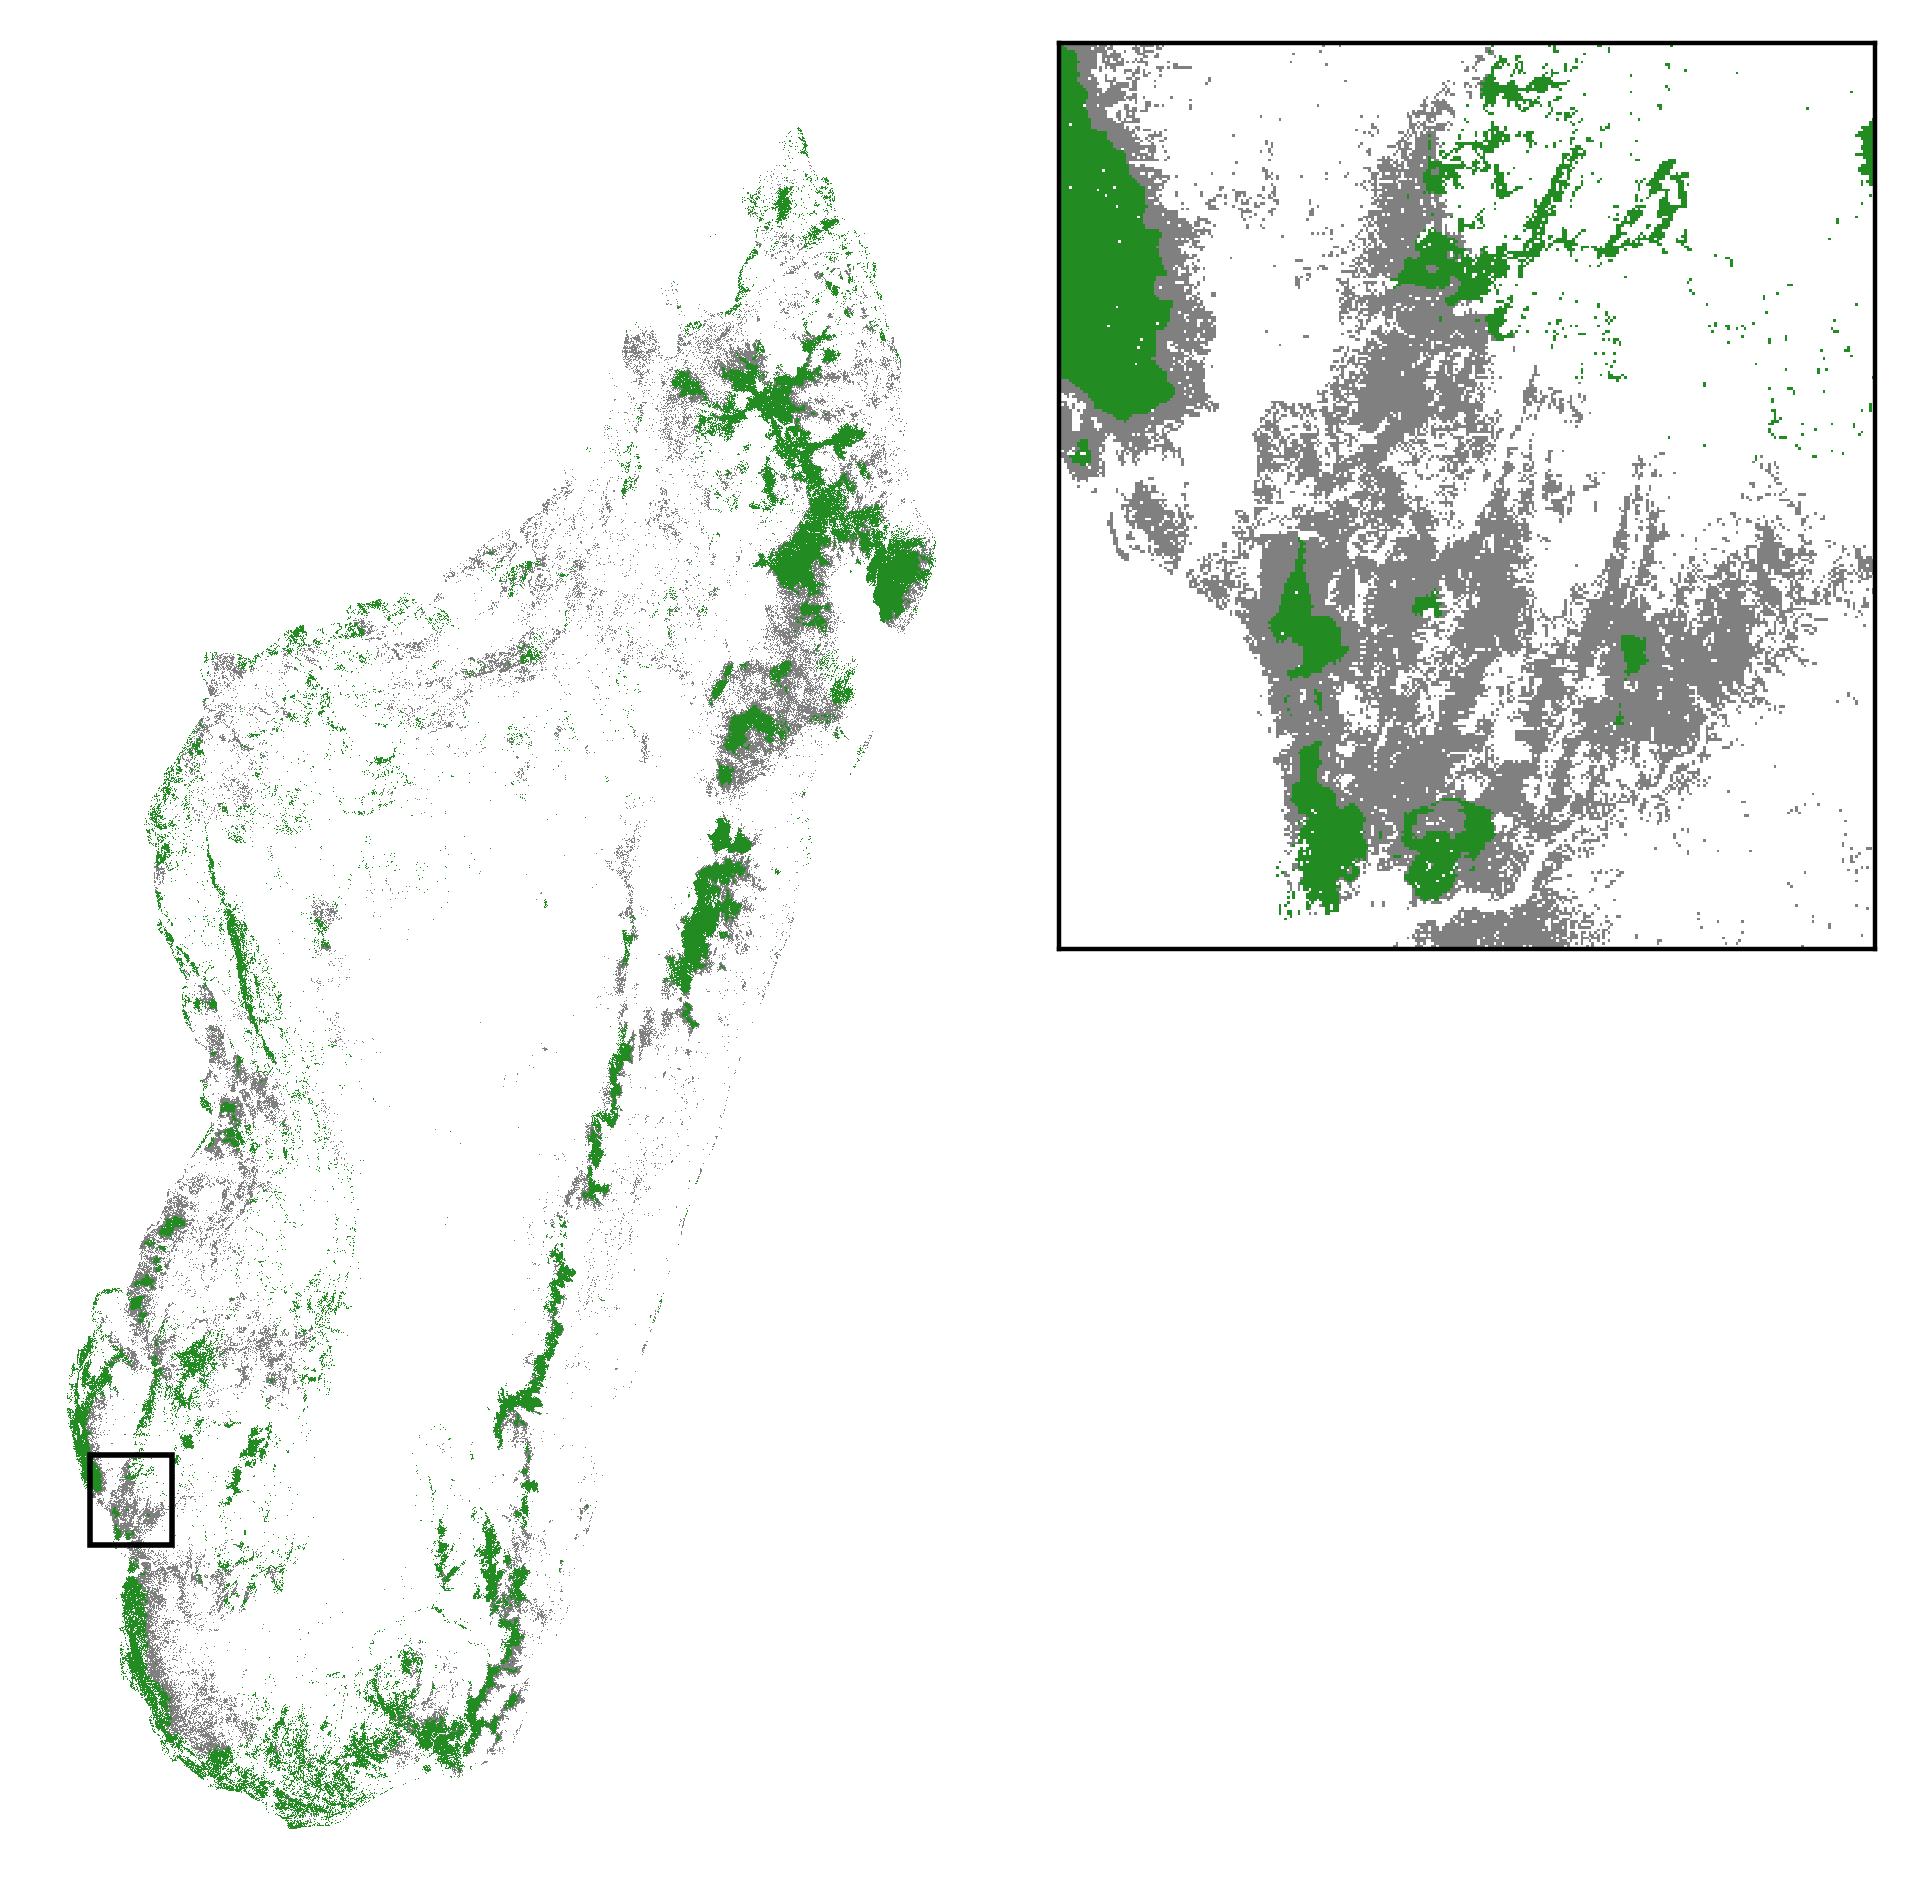
\includegraphics[width=\textwidth]{figures/forest_cover_2050} 

}

\caption{\textbf{Deforestation sur la période 2010-2050 et
couverture forestière en 2050 à Madagascar}. Nous projetons la
couverture forestière à l'horizon 2050 en considérant une déforestation
moyenne annuelle de 100~000 ha/an. Vert: forêt résiduelle en 2050; gris:
déforestation sur la période 2010-2050.}\label{fig:fc2050}
\end{figure}

\hypertarget{modeles-devolution-de-lintensite-de-deforestation-en-afrique-et-a-madagascar-1}{%
\paragraph{Modèles d'évolution de l'intensité de déforestation en
Afrique et à
Madagascar}\label{modeles-devolution-de-lintensite-de-deforestation-en-afrique-et-a-madagascar-1}}

Afin de proposer des scénarios d'évolution de l'intensité de
déforestation et du couvert forestier à Madagascar, il a fallu
construire un modèle à l'échelle de l'Afrique afin de disposer d'un plus
grand nombre de données et d'avoir un modèle plus robuste. Le modèle
permet d'estimer le taux de déforestation (en ha/an) pour l'ensemble des
pays africains en prenant en compte le couvert forestier existant (en
ha) et la taille de la population (en nombre d'habitants). Trois jeux de
données ont été comparés pour la modélisation : (i) celui issu du
rapport Global Forest Ressource Assessment (FRA) 2015 de la FAO (FAO
2015), (ii) celui issu du projet Trees du JRC (Frédéric Achard et al.
2014) et (iii) celui issu de Global Forest Watch (Hansen et al. 2013).
Nous montrons que les données de déforestation du FRA ne peuvent pas
être utilisées pour modéliser et prédire la déforestation (``outlier'').
Les résultats permettent également de montrer que malgré les variations
annuelles des taux de déforestation (associables aux marchés et aux
politiques), la tendance sur le long terme est forte et qu'un simple
modèle permet de reproduire fidèlement l'évolution du couvert forestier
de 1990 à 2015 pour la plupart des pays africains. Ce modèle est utilisé
pour prédire les tendances de déforestation pour les pays africains,
selon un scénario de référence (ou scénario ``business-as-usual''), en
tenant compte des projections démographiques des Nations Unies jusqu'à
l'horizon 2100. Pour Madagascar, on observerait une diminution de
l'intensité de déforestation après 1950 liée à la transition
démographique et à la réduction du couvert forestier disponible.
Toutefois, les surfaces déforestées annuellement resteraient importantes
(\textgreater{}75000 ha/an). Selon ce scénario, le couvert forestier
diminuerait ainsi de plus de 50\% entre 2000 et 2050 et de plus de 75\%
entre 2000 et 2100, pour atteindre environ 2 Mha en 2100
(Fig.~\ref{fig:intensity}). Ces scénarios d'évolution de l'intensité de
déforestation intégrant la croissance démographique seront utilisés pour
obtenir de nouvelles cartes du couvert forestier futur en 2050 et 2100.











\begin{figure}[H]

{\centering 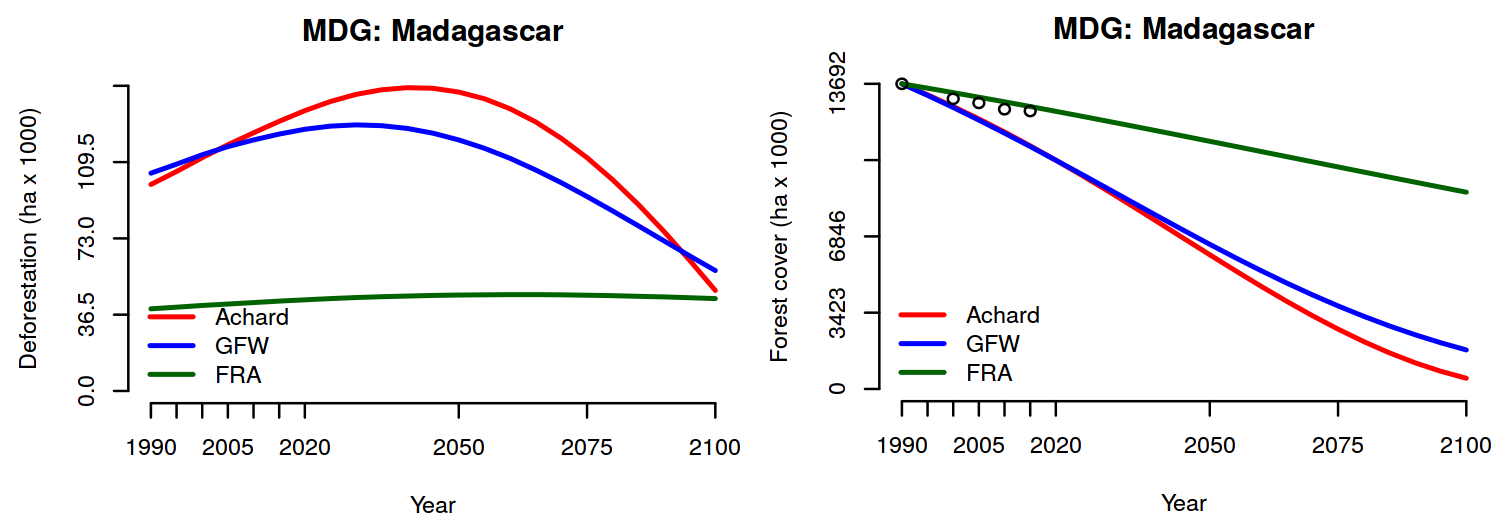
\includegraphics[width=\textwidth]{figures/deforMada} 

}

\caption{\textbf{Evolution (1990-2010) et prédiction
(2010-2100) de la déforestation et du couvert forestier à Madagascar.}
La figure de gauche montre l'évolution de la déforestation (en milliers
d'hectares par an) et la figure de droite l'évolution du couvert
forestier (en milliers d'hectares). Nous avons considéré trois jeux de
données (FAO FRA, Achard et al.~2014 JRC TREES project, Global Forest
Watch Hansen et al.~2013). Les projections prennent en compte la
croissance démographique (données des Nations Unies, 2015 Revision of
World Population Prospects).}\label{fig:intensity}
\end{figure}

\hypertarget{liste-des-publications-et-communications-scientifiques}{%
\subsection{\texorpdfstring{\emph{Liste des publications et
communications
scientifiques}}{Liste des publications et communications scientifiques}}\label{liste-des-publications-et-communications-scientifiques}}

\hypertarget{i.1---articles-ou-communications-primaires-resultats-originaux-scientifiques}{%
\subsubsection{I.1 - Articles ou communications primaires (résultats
originaux)
scientifiques}\label{i.1---articles-ou-communications-primaires-resultats-originaux-scientifiques}}

\hypertarget{i.1.1.-dans-periodique-a-comite-de-lecture.}{%
\paragraph{I.1.1. Dans périodique à comité de
lecture.}\label{i.1.1.-dans-periodique-a-comite-de-lecture.}}

\hypertarget{articles-acceptes}{%
\subparagraph{\texorpdfstring{\emph{Articles
acceptés}}{Articles acceptés}}\label{articles-acceptes}}

Dezécache C., J.-M. Salles, G. Vieilledent, and B. Hérault. 2017. Moving
forward socio-economically focused models of deforestation. \emph{Global
Change Biology}. 23(9): 3484-3500.
\url{https://doi.org.10.1111/gcb.13611}.

El Hajj M., N. Baghdadi, I. Fayad, G. Vieilledent, J.-S. Bailly, and D.
Ho Tong Minh. 2017. Interest of integrating spaceborne LiDAR data to
improve the estimation of biomass in high biomass forested areas.
\emph{Remote Sensing}. 9(3). \url{https://doi.org/10.3390/rs9030213}.

Vieilledent G., O. Gardi, C. Grinand, C. Burren, M. Andriamanjato, C.
Camara, C. J. Gardner, L. Glass, A. Rasolohery, H. Rakoto Ratsimba, V.
Gond, and J.-R. Rakotoarijaona. 2016. Bioclimatic envelope models
predict a decrease in tropical forest carbon stocks with climate change
in Madagascar. \emph{Journal of Ecology}. 104: 703-715. doi:
\url{https://doi.org/10.1111/1365-2745.12548}.

\hypertarget{articles-en-pre-printreview}{%
\subparagraph{\texorpdfstring{\emph{Articles en
pre-print/review}}{Articles en pre-print/review}}\label{articles-en-pre-printreview}}

Vieilledent G., C. Grinand, F. A. Rakotomalala, R. Ranaivosoa, J.-R.
Rakotoarijaona, T. F. Allnutt, and F. Achard. Combining global tree
cover loss data with historical national forest-cover maps to look at
six decades of deforestation and forest fragmentation in Madagascar.
\emph{bioRxiv}. 147827. doi: \url{https://doi.org/10.1101/147827}. in
review in \emph{Biological Conservation}.

\hypertarget{articles-en-preparation}{%
\subparagraph{\texorpdfstring{\emph{Articles en
préparation}}{Articles en préparation}}\label{articles-en-preparation}}

Charra M., S. Goodman, A. Raselimanana, M.-J. Raherilalao, V.
Soarimalala, D. Lees, F. Rakotondrainibe, J. Moat, M. Andriamanjato, W.
J. Baker, M. Rakotoarinivo, M. Vorontsova, T. Pearce, T. F. Allnutt, D.
Razafimpahanana, M. Pedrono, J.-R. Rakotoarijaona and G. Vieilledent.
Climate or watersheds ? Environmental factors determining species
assemblages change according to the taxonomic group. in prep.

Muniz-Tagliari M., J.-M. Leong Pock-Tsy, C. Cornu and P. Danthu and G.
Vieilledent. Vulnerability of the seven Madagascar's baobab species to
climate change. in prep.

Vieilledent G., M. Muniz-Tagliari, C. Grinand, F. Montfort. Atlas of the
biodiversity of Madagascar: present species distribution and species
vulnerability to climate change. in prep.

Vieilledent G., C. Grinand, M. Pedrono, T. Rabetrano, J.-R.
Rakotoarijaona, B. Rakotoarivelo, F. A. Rakotomalala, L. Rakotomalala,
A. Razafimpahanana, M. Nourtier, and F. Achard. It's not only poverty:
uncontrolled global trade and bad governance are responsible for rampant
deforestation in Western Madagascar. in prep.

Vieilledent G., and F. Achard. Including spatial-autocorrelation in
deforestation model to obtain realistic deforestation projections at
national or continental scales. in prep.

Grinand C., G. Vieilledent, T. Razafimbelo, J.-R. Rakotoarijaona, M.
Nourtier M., and M. Bernoux. Land use change spatial modeling using
machine learning tools and a global land cover change dataset. in prep.

Vieilledent G., W. F. Laurance, S. Peedell, and F. Achard. The fate of
tropical forests associated to the demographic explosion in Africa. in
prep.

Vieilledent G., 2016. MadaClim: a set of climatic and environmental
spatial variables for Madagascar. Data paper. in prep.

\hypertarget{i.1.2.-dans-periodique-sans-comite-de-lecture.}{%
\paragraph{I.1.2. Dans périodique sans comité de
lecture.}\label{i.1.2.-dans-periodique-sans-comite-de-lecture.}}

\hypertarget{i.1.3.-rapports-diplomants-master-these}{%
\paragraph{I.1.3. Rapports diplômants (Master,
Thèse)}\label{i.1.3.-rapports-diplomants-master-these}}

Grinand C. 2016. Suivi et modélisation des changements d'usage des
terres et stocks de carbone dans les sols et les arbres dans le cadre de
la REDD+ à Madagascar. Vers des mesures pertinentes localement et
cohérentes à large échelle. \emph{Thèse de doctorat en Écologie
Fonctionnelle et Sciences Agronomiques.} Montpellier SupAgro. Ecole
doctorale GAIA.

Muniz-Tagliari M. 2015. Biogéographie et vulnérabilité au changement
climatique des espèces de baobabs à Madagascar. \emph{Master II Biologie
Végétale Tropicale.} Université de Montpellier.

Charra M. 2015. Mise en place d'une base de données et réalisation d'une
carte de biodiversité faune/flore à Madagascar. \emph{Master II Ecologie
Biologie Evolution.} Université Paris-Sud XI, Orsay.

Long R. 2014. Modélisation de la déforestation à Madagascar.
\emph{Master I Agronomie Générale}. AgroParisTech.

\hypertarget{i.1.4.-communications-courtes-dans-congres-symposiums-scientifiques-preciser-le-support-ecrit-poster-resume-ou-texte-integral.}{%
\paragraph{I.1.4. Communications courtes dans congrès / symposiums
scientifiques (préciser le support écrit : poster, résumé ou texte
intégral).}\label{i.1.4.-communications-courtes-dans-congres-symposiums-scientifiques-preciser-le-support-ecrit-poster-resume-ou-texte-integral.}}

Vieilledent G., W. F. Laurance, S. Peedell, and F. Achard. The fate of
tropical forests associated to the demographic explosion in Africa.
Scennet 2016: international conference on Scenarios and Models of
Biodiversity and Ecosystem Services in Support of Decision Making.
Montpellier. Présentation orale.

Grinand C., G. Vieilledent, T. Razafimbelo, J.-R. Rakotoarijaona, M.
Nourtier M., and M. Bernoux. 2016. New tools and methodological
framework to study spatial drivers of deforestation, degradation and
regeneration and forecast possible futures in Madagascar. Scennet 2016:
international conference on Scenarios and Models of Biodiversity and
Ecosystem Services in Support of Decision Making. Montpellier.
Présentation orale.

Vieilledent G., O. Gardi, C. Grinand, C. Burren, M. Andriamanjato, C.
Camara, C. J. Gardner, L. Glass, A. Rasolohery, H. Rakoto Ratsimba, V.
Gond, J.-R. Rakotoarijaona. 2016. Bioclimatic envelope models predict a
decrease in tropical forest carbon stocks with climate change in
Madagascar. In : Tropical ecology and society reconciliating
conservation and sustainable use of biodiversity. Program and abstracts.
Plinio Sist (ed.), Stéphanie Carrière (ed.), Pia Parolin (ed.),
Pierre-Michel Forget (ed.). ATBC. Storrs : ATBC, Résumé, p.~325.
Montpellier. Présentation orale.

Vieilledent G., M. Charra, M. Muniz-Tagliari, C. Grinand, T. F. Allnutt,
D. Razafimpahanana, M. Pedrono, J.-R. Rakotoarijaona. 2015. Biodiversity
Scenarios in Madagascar. ICCB-ECCB 2015: 27th International Congress for
Conservation Biology - 4th European Congress for Conservation Biology
conference. Montpellier. Poster.

Vieilledent G., T. F. Allnutt, C. Grinand, M. Pedrono, J.-R.
Rakotoarijaona, and D. Razafimpahanana. BioSceneMada: Biodiversity
scenarios under the effect of climate change and future deforestation in
Madagascar. ICCB-ECCB 2015: 27th International Congress for Conservation
Biology - 4th European Congress for Conservation Biology conference.
Montpellier. Side-event FRB-FFEM. Présentation orale.

Vieilledent G., and F. Achard. 2018. Accounting for spatial
autocorrelation in deforestation modelling. ISEC 2018: International
Statistical Ecology Conference. St Andrews (UK). Présentation orale.

\hypertarget{i.1.5.-autres-supports.}{%
\paragraph{I.1.5. Autres supports.}\label{i.1.5.-autres-supports.}}

Vieilledent G., C. Grinand, M. Pedrono, T. Rabetrano, J.-R.
Rakotoarijaona, B. Rakotoarivelo, F. A. Rakotomalala and Dimby
Razafimpahanana. 2016. Deforestation process in the dry forests of the
Menabe region, western Madagascar. Mission report.

\hypertarget{i.2---syntheses-scientifiques}{%
\subsubsection{I.2 - Synthèses
scientifiques}\label{i.2---syntheses-scientifiques}}

I.2.1. Dans périodique à comité de lecture.\\
I.2.2. Dans périodique sans comité de lecture. I.2.3. Chapitre
d'ouvrage.\\
I.2.4. Ouvrage entier.\\
I.2.5. Rapports diplômants à caractère bibliographique (thèse
vétérinaire\ldots{}).\\
I.2.6. Conférences dans congrès ou symposium scientifique. I.2.7. Autres
supports.

\newpage

\hypertarget{tableau-des-livrables}{%
\subsection{\texorpdfstring{\emph{Tableau des
livrables}}{Tableau des livrables}}\label{tableau-des-livrables}}






\label{tab:livrables}\textbf{Livrables du projet BioSceneMada.} Les
livrables sont classés par catégories (``Bases de données'', ``Cartes'',
etc.). Les articles, disposant d'une section spécifique dans le rapport,
n'ont pas été repris.

Catégorie

Description

Commentaire

Bases de données

Variables climatiques et environnementales

Livré

Inventaires de 1771 placettes pour le stock de carbone forestier

Livré

Base de données de biodiversité (points de présence pour 4969 espèces)

Livré

Scénarios

Scénarios de déforestation: tendance historique et effet de la
démographie

Livré

Scénarios climatiques et biodiversité

Livré pour certains groupes taxonomiques. A généraliser à l'ensemble des
espèces.

Cartes

Evolution (1953-2014) du couvert forestier (30m)

Livré

Carte de probabilité de déforestation (30m)

Livré

Couvert forestier futur en 2050 et 2100 (30m)

Livré pour 2050. En cours pour 2100. Inclure le scénario avec croissance
démographique.

Stocks de carbone forestier en 2010 et 2080 (250m)

Livré

Cartes des habitats forestiers vulnérables/résilients aux changement
climatiques

Livré

Carte de biodiversité beta (1km)

Première version. Nouvelle approche à développer pour tenir compte des
différences entre groupes taxonomiques.

Atlas

Atlas de la biodiversité à Madagascar

Prototype livré. A généraliser à l'ensemble des espèces

Logiciels

Module Python `deforestprob' pour la modélisation de la déforestation

Livré

Script R `atlas' pour la modélisation de la niche climatique des espèces

Livré

\newpage

\hypertarget{personnes-ayant-participe-a-ce-projet}{%
\subsection{\texorpdfstring{\emph{Personnes ayant participé à ce
projet}}{Personnes ayant participé à ce projet}}\label{personnes-ayant-participe-a-ce-projet}}

\begin{tabular}{lllllllll}
\toprule
Institut & Nom & Statut particulier\\
\midrule
ONE & Jean-Roger Rakotoarijaona & \\
 & Rija Ranaivosoa & \\
 & Bruno Rakotoarivelo & \\
ETC Terra & Clovis Grinand & Thésard\\
 & Fety A. Rakotomalala & \\
\addlinespace
 & Marie Nourtier & \\
 & Frédérique Montfort & \\
 & Ruoyin Long & Stagiaire\\
WCS & Andriamandimbisoa (Dimby) Razafimpahanana & \\
 & Thomas F. Allnutt & \\
\addlinespace
 & Tsiky Rabetrano & \\
Cirad & Ghislain Vieilledent & \\
 & Miguel Pedrono & \\
 & Mario Muniz-Tagliari & Stagiaire\\
 & Margaux Charra & Stagiaire\\
\bottomrule
\end{tabular}

\hypertarget{autres-actions-produits-de-diffusion-et-exploitation-des-resultats-vers-les-decideurs-et-les-acteurs-concernes}{%
\section{5. Autres actions, produits de diffusion et exploitation des
résultats vers les décideurs et les acteurs
concernés}\label{autres-actions-produits-de-diffusion-et-exploitation-des-resultats-vers-les-decideurs-et-les-acteurs-concernes}}

\hypertarget{diffusion-communication-et-transfert-de-connaissance-autres-que-supports-a-caractere-scientifique}{%
\subsection{Diffusion, communication et transfert de connaissance
(autres que supports à caractère
scientifique)}\label{diffusion-communication-et-transfert-de-connaissance-autres-que-supports-a-caractere-scientifique}}

\hypertarget{sites-internet}{%
\subsubsection{Sites internet}\label{sites-internet}}

Site web du projet BioSceneMada (\url{https://bioscenemada.cirad.fr}).
Le site web permet d'avoir accès à toutes les informations et documents
relatifs au déroulement du projet.

Le site web MadaClim (\url{https://madaclim.cirad.fr}), produit du
projet BioSceneMada, regroupe les données climatiques et
environnementales pour Madagascar.

\hypertarget{presentations}{%
\subsubsection{Présentations}\label{presentations}}

M. Pedrono, T. F. Allnutt, C. Grinand, J.-R. Rakotoarijaona, D.
Razafimpahanana, and G. Vieilledent. Séminaire du projet FED-FEDER POCT
``Biodiversité de l'Océan Indien''``, 2-5 juin 2015, Université de la
Réunion, Saint Denis, Réunion, France. Public: Experts de la
biodiversité de l'Océan Indien continental et étudiants en écologie de
la Réunion.

Vieilledent G., T. F. Allnutt, C. Grinand, M. Pedrono, J.-R.
Rakotoarijaona, and D. Razafimpahanana. 2015. BioSceneMada: Scénarios de
la biodiversité sous l'effet conjoint du changement climatique et de la
déforestation à Madagascar. Journées FRB 2015, ``Les scénarios de la
biodiversité à l'heure du changement climatique''. 2 octobre 2015.
Paris. Public: Experts français de l'IPBES et du GIECC.

M. Pedrono, T. F. Allnutt, C. Grinand, J.-R. Rakotoarijaona, D.
Razafimpahanana, and G. Vieilledent. Journée d'animation scientifique du
Dispositif en Partenariat ``Forêt et Biodiversité'', 25 septembre 2015,
FOFIFA-DRFP, Antananarivo, Madagascar. Public: Chercheurs et étudiants
malgaches, membres de la direction du CIRAD.

M. Pedrono, T. F. Allnutt, C. Grinand, J.-R. Rakotoarijaona, D.
Razafimpahanana, and G. Vieilledent. Table ronde de la Journée du
Volontariat Français sur le thème ``Regards croisés sur le changement
climatique à Madagascar'', 3 octobre 2015, Alliance Française,
Antananarivo, Madagascar. Public: Grand public malgache et français,
volontaires internationaux français, ONGs de développement.

M. Pedrono, T. F. Allnutt, C. Grinand, J.-R. Rakotoarijaona, D.
Razafimpahanana, and G. Vieilledent. Série de conférences ``COP21 à
l'Institut Français de Madagascar: la recherche et le changement
climatique'', 25 novembre 2015, Alliance Française, Antananarivo,
Madagascar. Public: Grand public malgache et français.

\hypertarget{reunions-avec-les-parties-prenantes}{%
\subsubsection{Réunions avec les
parties-prenantes}\label{reunions-avec-les-parties-prenantes}}

Plusieurs réunions de présentation du projet et de présentation des
résultats intermédiaires ont eu lieu à Antananarivo avec les
parties-prenantes du projet. Etaient présents des membres du MEEF
(Ministère de l'Environnement, de l'Ecologie et des Forêts, Direction
Générale des Forêts et Direction Générale de l'Environnement), des ONG
environnementales (WWF, WCS, CI, GERP, Asity Madagascar, Vahatra,
Biotope, Blue Ventures), des chercheurs (Université d'Antananarivo,
ESSA, IOGA, LRI, IRD, Cirad, RGB Kew, MBG), des membres d'institutions
nationales (Madagascar National Park, Office National de
l'Environnement, FOFIFA):

\begin{itemize}
\tightlist
\item
  Réunion de présentation des avancées du projet, le 3 Juin 2016 à
  Antananarivo
\item
  Réunion de présentation des avancées du projet, le 2 Avril 2015 à
  Antananarivo
\item
  Réunion de lancement du projet, le 5 Mars 2014 à Antananarivo
\end{itemize}






\begin{figure}[H]

{\centering 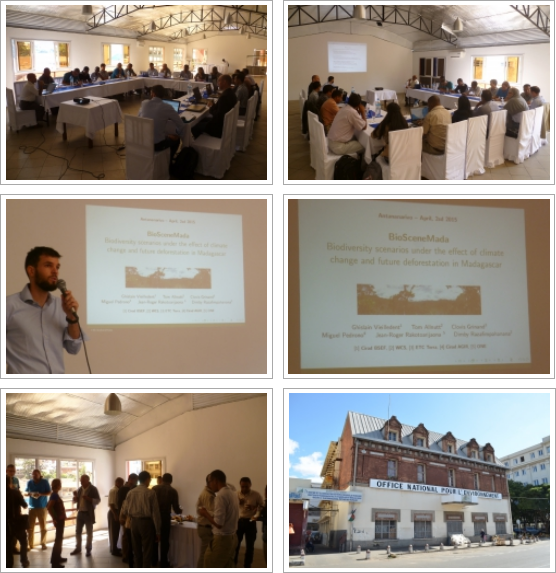
\includegraphics[width=\textwidth]{figures/Meeting} 

}

\caption{\textbf{Participants à la réunion de présentation des
avancées du projet, le 3 Juin 2016 à Antananarivo.} Les participants
incluent des chercheurs, étudiants, membres d'ONG environnementales ou
institutions nationales.}\label{fig:meeting}
\end{figure}

\hypertarget{articles-de-presse}{%
\subsubsection{Articles de presse}\label{articles-de-presse}}

Les résultats de l'article sur la vulnérabilité des forêts tropicales au
changement climatique à Madagascar ont été largement diffusés dans la
presse:
\href{https://jecologyblog.wordpress.com/2016/05/06/editors-choice-1043/}{Journal
of Ecology's blog}, \href{https://t.co/pMXLUUrV0I}{The Conversation},
\href{https://ghislainv.github.io/images/media/Figaro-16-02-2016.png}{Le
Figaro},
\href{http://www.lepoint.fr/environnement/le-rechauffement-climatique-risque-d-empecher-les-forets-tropicales-de-stocker-le-carbone-12-02-2016-2017587_1927.php\#xtor=RSS-221}{Le
Point},
\href{http://www.francetvinfo.fr/monde/environnement/le-rechauffement-climatique-risque-d-empecher-les-forets-tropicales-de-stocker-le-carbone_1312341.html\#xtor=AL-54-\%5Barticle\%5D}{FranceTV
info},
\href{http://www.emol.com/noticias/Tecnologia/2016/02/12/788109/Estudio-asegura-que-cambio-climatico-amenaza-la-absorcion-de-CO2-por-bosques-tropicales.html}{El
Mercurio},
\href{https://ghislainv.github.io//images/media/MidiLibre-16-02-2016.png}{Midi-Libre},
\href{http://www.cirad.fr/en/news/all-news-items/press-releases/2016/climate-change-alters-the-co2-storage-capacity-of-tropical-forests}{Cirad},
\href{https://www.cirad.fr/content/download/11005/128917/version/3/file/RA2015_FR.pdf}{Cirad
activity report 2015}.

\hypertarget{interviews}{%
\subsubsection{Interviews}\label{interviews}}

Les résultats de l'article sur la vulnérabilité des forêts tropicales au
changement climatique à Madagascar ont fait l'objet d'une interview sur
Radio Classique dans l'émission ``3 minutes pour la planète'' du 16
Février 2016.

\hypertarget{outils-de-gestion-ou-daide-a-la-decision-developpes-grace-a-ce-projet}{%
\subsection{Outils de gestion ou d'aide à la décision développés grâce à
ce
projet}\label{outils-de-gestion-ou-daide-a-la-decision-developpes-grace-a-ce-projet}}

Plusieurs outils ont été développés au cours du projet BioSceneMada pour
la gestion ou l'aide à la décision concernant la conservation de la
biodiversité à Madagascar. Ces outils sont sous forme de bases de
données, de cartes à haute résolution, d'un atlas de la biodiversité, de
logiciels. Ces outils seront notamment utiles pour l'application du
programme REDD+ à Madagascar et l'optimisation du réseau d'aires
naturelles protégées.

\emph{Base de données}: Le projet BioSceneMada a permis de constituter
une base de données climatiques et environnementales à Madagascar. Le
projet a également permis d'obtenir une base de données de biodiversité
incluant plus de 300 000 points de présences pour 4969 espèces
représentatives de la biodiversité à Madagascar. Cette base de données,
incluant des données privées, sera accessible sur demande.

\emph{Cartes}: Le projet BioSceneMada a permis d'obtenir différentes
cartes utiles pour la gestion de la biodiversité. Sont disponibles: des
cartes de couverts forestiers sur la période 1953-2014 à 30m de
résolution, une première carte de la biodiversité \(\beta\), une carte
des habitats forestiers vulnérables/résilients aux changements
climatiques, une carte de la couverture forestière probable en 2050 et
2100 indiquant les zones à risque de déforestation.

\emph{Atlas}: Un atlas de la biodiversité est en cours de réalisation.
Un prototype de cet atlas a déjà été réalisé pour le groupe des baobabs
à Madagascar. Cet atlas permettra d'obtenir l'aire de distribution
actuelle des espèces ainsi qu'une estimation de leur vulnérabilité au
changement climatique indiquant notamment les zones de refuge climatique
pour ces espèces.

\emph{Bibliothèques logicielles}: Deux principales bibliothèques
logicielles à destination des gestionnaires ont été développées au cours
du projet. Le module Python \texttt{deforestprob} permet la modélisation
et la projection spatialisée de la déforestation dans le futur suivant
différents scénarios d'intensité. Le script R \texttt{atlas} permet de
modéliser la niche climatique des espèces et leur vulnérabilité au
changement climatique en fonction des données de présence de l'espèce.

\hypertarget{activites-de-suivi-et-projets-de-valorisation-des-resultats}{%
\subsection{Activités de suivi et projets de valorisation des
résultats}\label{activites-de-suivi-et-projets-de-valorisation-des-resultats}}

Sur 2018 et 2019, les deux dernières années du projet, il est prévu
d'organiser des ateliers de renforcement de capacité à Madagascar. Ces
ateliers seront à destination des étudiants, chercheurs, techniciens et
gestionnaires à Madagascar travaillant sur la conservation de la
biodiversité. Le renforcement de capacité porterait sur les approches et
outils développés au cours du projet BioSceneMada, à savoir: (i) sur les
modèles de déforestation et les scénarios de référence, (ii) sur les
modèles de niche et l'atlas, (iii) sur les modèles de communauté et la
réalisation de cartes de biodiversité.

Le premier atelier de renforcement de capacité sur les modèles de
déforestation aura pour objectif de former les participants à
l'utilisation du module Python \texttt{deforestprob}, servant à la
spatialisation et la projection de la déforestation. Différents
scénarios d'intensité de déforestation pourront être explorés. Les
cartes de couvert forestier futur produites par les participants
pourront être utilisées pour l'établissement du scénario de référence
concernant les émissions de CO\textsubscript{2} associées à la
déforestation à Madagascar. Ce scénario à l'échelle nationale est
important pour la mise en place du programme REDD+ (``Réduction des
Emissions liées à la Déforestation et la Dégradation des forêts'') à
Madagascar. Les membres du ``Bureau National REDD+'' seront invités à
participer à cette formation. L'objectif est que les participants
puissent mettre à jour le scénario de référence au fur et à mesure de
l'actualisation des cartes historiques de déforestation ou des variables
explicatives en entrée (développement du réseau routier par exemple).

Un second atelier de renforcement de capacité sera organisé sur les
modèles de niche climatique. Ce second atelier aura pour objectif de
former les participants à l'utilisation du script R permettant
l'obtention des fiches par espèce constituant l'atlas de la biodiversité
à Madagascar. L'objectif est que les participants puissent mettre à jour
les fiches espèces et l'atlas au fur et à mesure de l'actualisation des
données de présence. Ces fiches peuvent être utilisées afin d'identifier
les espèces présentes sur un territoire (une aire protégée par exemple)
et d'estimer la vulnérabilité de ces espèces au changement climatique
afin d'entreprendre d'éventuelles actions de conservation. Ces actions
de conservation peuvent inclure des actions de protection
supplémentaires pour certaines zones refuges de la biodiversité ou de la
restauration d'habitat. Il nous semble que ces outils seraient
particulièrement utiles aux gestionnaires d'aires protégées à
Madagascar. Les gestionnaires d'aires protégées comme Madagascar
National Park seront invités à participer à cet atelier. L'ONE est
également demandeur de ces outils afin de pouvoir obtenir des listes de
présence d'espèces sur une zone donnée pour les études d'impact et les
autorisations d'exploitation des ressources naturelles notamment.

En fonction du temps et du budget, un troisième atelier sera organisé
sur les modèles de communauté et la réalisation de cartes de
biodiversité à Madagascar. Enfin, une réunion de présentation des
résultats consolidés du projet sera organisée à Antananarivo en 2019.
L'ensemble des parties-prenantes du projet, travaillant dans le domaine
de l'environnement à Madagascar, sera invité à participer à cette
réunion.

\hypertarget{acces-aux-donnees}{%
\section{6. Accès aux données}\label{acces-aux-donnees}}

\hypertarget{donnees}{%
\subsection{Données}\label{donnees}}

Un effort a été entrepris afin que les données du projet soient rendues
disponibles gratuitement et de façon permanente avec l'attribution d'un
DOI (Digital Object Identifier) unique. Les plateformes utilisées pour
l'archivage des données sont actuellement soit Dryad
(\url{https://datadryad.org}), soit Zenodo (\url{https://zenodo.org}). A
terme, l'ensemble des données sera disponible sur la plateforme
Dataverse du Cirad (\url{https://dataverse.cirad.fr}), qui a été lancée
en Février 2018. C'est le lien vers la plateforme Dataverse qui sera
préférentiellement utilisé dans les publications. D'autres données
seront rendues publiques au fur et à mesure de la publication des
articles en préparation.

\begin{itemize}
\tightlist
\item
  Base de données climatiques et environnementales MadaClim accessible
  via le site internet \url{https://madaclim.cirad.fr}.
\item
  Carte des stocks de carbone forestier sur le site internet du projet à
  l'adresse \url{https://bioscenemada.cirad.fr/carbonmaps}, ainsi que
  sur la plateforme Dryad \url{https://doi.org/10.5061/dryad.9ph68}.
\item
  Cartes de couverture forestière sur la période 1953-2014 accessibles
  sur le site internet du projet à l'adresse
  \url{https://bioscenemada.cirad.fr/forestmaps}, ainsi que sur la
  plateforme Zenodo \url{https://doi.org/10.5281/zenodo.1145785}.
\item
  Carte de probabilité de déforestation en 2010 sur le site du projet:
  \url{https://bioscenemada.cirad.fr/forestmaps}
\item
  Carte de couvert forestier futur pour l'année 2050:
  \url{https://bioscenemada.cirad.fr/forestmaps}
\end{itemize}

Concernant la base de données de biodiversité, les données qu'elle
inclue proviennent d'institutions différentes qui ont accepté de les
partager dans le cadre du projet BioSceneMada. Seule une partie de ces
données brutes sont accessibles publiquement. Une discussion avec
l'ensemble des institutions ayant fourni les données de biodiversité
aura lieu d'ici la fin du projet afin de voir dans quelle mesure
celles-ci peuvent être rendues publiques à l'issue du projet. Les
données de biodiversité publiques seront regroupées et rendues
accessibles dès leur valorisation à travers la publication des articles
en préparation.

\hypertarget{scripts-informatiques}{%
\subsection{Scripts informatiques}\label{scripts-informatiques}}

La plupart des scripts informatiques ayant servi à l'obtention des
résultats sont également mis à la disposition de la communauté
scientifique et des gestionnaires. L'outil utilisé pour le partage du
code est la plateforme GitHub. Comme pour les données, d'autres
répertoires seront créés et rendus publiques au fur et à mesure de la
publication des articles en préparation.

\begin{itemize}
\tightlist
\item
  Code pour les données climatiques et environnementales:
  \url{http://ghislainv.github.io/madaclim}
\item
  Code pour les stocks de carbone forestiers:
  \url{https://github.com/ghislainv/carbonmap}
\item
  Code du module Python \texttt{deforestprob}:
  \url{https://github.com/ghislainv/deforesprob}
\item
  Code pour les cartes historiques de déforestation sur la période
  1953-2014: \url{https://github.com/ghislainv/deforestation-maps-Mada}
\item
  Code pour la carte de probabilité de déforestation et la carte de
  couvert forestier en 2050:
  \url{https://ghislainv.github.io/deforestprob}
\item
  Code pour l'atlas de biodiversité:
  \url{https://github.com/ghislainv/atlas} (accès privé pour le moment,
  couple identifiant/mot de passe: \texttt{gvguest}/\texttt{gvguest!1})
\item
  Code pour l'analyse de la déforestation dans le Menabe:
  \url{https://github.com/ghislainv/menabe}
\end{itemize}

\hypertarget{references}{%
\section{7. Références}\label{references}}

\hypertarget{refs}{}
\leavevmode\hypertarget{ref-Achard2002}{}%
Achard, F., H. D. Eva, H. J. Stibig, P. Mayaux, J. Gallego, T. Richards,
and J. P. Malingreau. 2002. ``Determination of Deforestation Rates of
the World's Humid Tropical Forests.'' \emph{Science} 297
(5583):999--1002.

\leavevmode\hypertarget{ref-Achard2014}{}%
Achard, Frédéric, René Beuchle, Philippe Mayaux, Hans-Jürgen Stibig,
Catherine Bodart, Andreas Brink, Silvia Carboni, et al. 2014.
``Determination of Tropical Deforestation Rates and Related Carbon
Losses from 1990 to 2010.'' \emph{Global Change Biology} 20
(8):2540--54. \url{https://doi.org/10.1111/gcb.12605}.

\leavevmode\hypertarget{ref-Ali2008}{}%
Ali, Jason R, and Jonathan C Aitchison. 2008. ``Gondwana to Asia: Plate
Tectonics, Paleogeography and the Biological Connectivity of the Indian
Sub-Continent from the Middle Jurassic Through Latest Eocene (166--35
Ma).'' \emph{Earth-Science Reviews} 88 (3). Elsevier:145--66.

\leavevmode\hypertarget{ref-Allnutt2008}{}%
Allnutt, Thomas F., Simon Ferrier, Glenn Manion, George V. N. Powell,
Taylor H. Ricketts, Brian L. Fisher, Grady J. Harper, et al. 2008. ``A
Method for Quantifying Biodiversity Loss and Its Application to a
50-Year Record of Deforestation Across Madagascar.'' \emph{Conservation
Letters} 1 (4). Blackwell Publishing Inc:173--81.
\url{http://dx.doi.org/10.1111/j.1755-263X.2008.00027.x}.

\leavevmode\hypertarget{ref-Andriamasimanana2013}{}%
Andriamasimanana, Rado H., and Alison Cameron. 2013. ``Predicting the
Impacts of Climate Change on the Distribution of Threatened
Forest-Restricted Birds in Madagascar.'' \emph{Ecol Evol} 3 (4):763--69.
\url{http://dx.doi.org/10.1002/ece3.497}.

\leavevmode\hypertarget{ref-Araujo2007a}{}%
Araujo, Miguel B., and Mark New. 2007. ``Ensemble Forecasting of Species
Distributions.'' \emph{Trends in Ecology \& Evolution} 22 (1):42--47.
\url{https://doi.org/10.1016/j.tree.2006.09.010}.

\leavevmode\hypertarget{ref-Brooks2006}{}%
Brooks, T. M., R. A. Mittermeier, G. A. B. da Fonseca, J. Gerlach, M.
Hoffmann, J. F. Lamoreux, C. G. Mittermeier, J. D. Pilgrim, and A. S. L.
Rodrigues. 2006. ``Global Biodiversity Conservation Priorities.''
\emph{Science} 313 (5783):58--61.

\leavevmode\hypertarget{ref-Burney2004}{}%
Burney, David A, Lida Pigott Burney, Laurie R Godfrey, William L
Jungers, Steven M Goodman, Henry T Wright, and AJ Jull. 2004. ``A
Chronology for Late Prehistoric Madagascar.'' \emph{Journal of Human
Evolution} 47 (1). Elsevier:25--63.

\leavevmode\hypertarget{ref-Cox2012}{}%
Cox, Murray P, Michael G Nelson, Meryanne K Tumonggor, François-Xavier
Ricaut, and Herawati Sudoyo. 2012. ``A Small Cohort of Island Southeast
Asian Women Founded Madagascar.'' \emph{Proceedings of the Royal Society
B: Biological Sciences} 279 (1739). The Royal Society:2761--8.

\leavevmode\hypertarget{ref-Crottini2012}{}%
Crottini, Angelica, Ole Madsen, Celine Poux, Axel Strauß, David R
Vieites, and Miguel Vences. 2012. ``Vertebrate Time-Tree Elucidates the
Biogeographic Pattern of a Major Biotic Change Around the K--T Boundary
in Madagascar.'' \emph{Proceedings of the National Academy of Sciences}
109 (14). National Acad Sciences:5358--63.

\leavevmode\hypertarget{ref-Dransfield1995}{}%
Dransfield, John, and Henk Beentje. 1995. \emph{The Palms of
Madagascar.} Royal Botanic Gardens.

\leavevmode\hypertarget{ref-FAO2015}{}%
FAO. 2015. ``Global Forest Resources Assessment 2015.'' Food;
Agriculture Organization of the United Nations.
\url{http://www.fao.org/fileadmin/user_upload/FRA/spreadsheet/FRA_data/BULK.zip}.

\leavevmode\hypertarget{ref-Ferrier2007}{}%
Ferrier, Simon, Glenn Manion, Jane Elith, and Karen Richardson. 2007.
``Using Generalized Dissimilarity Modelling to Analyse and Predict
Patterns of Beta Diversity in Regional Biodiversity Assessment.''
\emph{Diversity and Distributions} 13 (3). Wiley Online Library:252--64.

\leavevmode\hypertarget{ref-Goodman2005}{}%
Goodman, S. M., and J. P. Benstead. 2005. ``Updated Estimates of Biotic
Diversity and Endemism for Madagascar.'' \emph{Oryx} 39 (1):73--77.

\leavevmode\hypertarget{ref-Hannah2008}{}%
Hannah, L., R. Dave, P. P. Lowry, S. Andelman, M. Andrianarisata, L.
Andriamaro, A. Cameron, et al. 2008. ``Climate change adaptation for
conservation in Madagascar.'' \emph{Biology Letters} 4 (5):590--94.

\leavevmode\hypertarget{ref-Hansen2013}{}%
Hansen, M. C., P. V. Potapov, R. Moore, M. Hancher, S. A. Turubanova, A.
Tyukavina, D. Thau, et al. 2013. ``High-Resolution Global Maps of
21st-Century Forest Cover Change.'' \emph{Science} 342 (6160):850--53.
\url{https://doi.org/10.1126/science.1244693}.

\leavevmode\hypertarget{ref-Harper2007}{}%
Harper, G. J., M. K. Steininger, C. J. Tucker, D. Juhn, and F. Hawkins.
2007. ``Fifty years of deforestation and forest fragmentation in
Madagascar.'' \emph{Environmental Conservation} 34 (4):325--33.
\url{https://doi.org/10.1017/S0376892907004262}.

\leavevmode\hypertarget{ref-Holt2013}{}%
Holt, Ben G., Jean-Philippe Lessard, Michael K. Borregaard, Susanne A.
Fritz, Miguel B. Araujo, Dimitar Dimitrov, Pierre-Henri Fabre, et al.
2013. ``An Update of Wallace's Zoogeographic Regions of the World.''
\emph{Science} 339 (6115):74--78.

\leavevmode\hypertarget{ref-IPCC2007}{}%
IPCC. 2007. ``Fourth Assessment Report (AR4), Climate Change 2007:
Synthesis Report.'' The Intergovernmental Panel on Climate Change, IPCC.

\leavevmode\hypertarget{ref-Kremen2008}{}%
Kremen, C., A. Cameron, A. Moilanen, S. J. Phillips, C. D. Thomas, H.
Beentje, J. Dransfield, et al. 2008. ``Aligning Conservation Priorities
Across Taxa in Madagascar with High-Resolution Planning Tools.''
\emph{Science} 320 (5873):222--26.

\leavevmode\hypertarget{ref-Loarie2009}{}%
Loarie, S. R., P. B. Duffy, H. Hamilton, G. P. Asner, C. B. Field, and
D. D. Ackerly. 2009. ``The Velocity of Climate Change.'' \emph{Nature}
462 (7276):1052--5.

\leavevmode\hypertarget{ref-Menendez2006}{}%
Menéndez, Rosa, Adela González Megías, Jane K Hill, Brigitte Braschler,
Stephen G Willis, Yvonne Collingham, Richard Fox, David B Roy, and Chris
D Thomas. 2006. ``Species Richness Changes Lag Behind Climate Change.''
\emph{Proceedings of the Royal Society B: Biological Sciences} 273
(1593). The Royal Society:1465--70.

\leavevmode\hypertarget{ref-Mercier2013}{}%
Mercier, Jean-Luc, and Lucienne Wilmé. 2013. ``The Eco-Geo-Clim Model:
Explaining Madagascar's Endemism.'' \emph{Madagascar Conservation \&
Development} 8 (2). Indian Ocean e-Ink:63--68.

\leavevmode\hypertarget{ref-Myers2000}{}%
Myers, N., R. A. Mittermeier, C. G. Mittermeier, G. A. B. da Fonseca,
and J. Kent. 2000. ``Biodiversity Hotspots for Conservation
Priorities.'' \emph{Nature} 403 (6772):853--58.

\leavevmode\hypertarget{ref-Pearson2009}{}%
Pearson, Richard G, and Christopher J Raxworthy. 2009. ``The Evolution
of Local Endemism in Madagascar: Watershed Versus Climatic Gradient
Hypotheses Evaluated by Null Biogeographic Models.'' \emph{Evolution} 63
(4). Wiley Online Library:959--67.

\leavevmode\hypertarget{ref-Pekel2016}{}%
Pekel, Jean-François, Andrew Cottam, Noel Gorelick, and Alan S. Belward.
2016. ``High-Resolution Mapping of Global Surface Water and Its
Long-Term Changes.'' \emph{Nature} 540 (7633). Macmillan Publishers
Limited, part of Springer Nature. All rights reserved.:418--22.
\url{http://dx.doi.org/10.1038/nature20584}.

\leavevmode\hypertarget{ref-Rabearivony2010}{}%
Rabearivony, J., R. Thorstrom, L. A. R. de Roland, M. Rakotondratsima,
T. R. A. Andriamalala, T. S. Sam, G. Razafimanjato, D. Rakotondravony,
A. P. Raselimanana, and M. Rakotoson. 2010. ``Protected Area Surface
Extension in Madagascar: Do Endemism and Threatened Species Remain
Useful Criteria for Site Selection?'' \emph{Madagascar Conservation and
Development} 5 (1):35--47.

\leavevmode\hypertarget{ref-Raftery2012}{}%
Raftery, Adrian E., Nan Li, Hana Sevcikova, Patrick Gerland, and Gerhard
K. Heilig. 2012. ``Bayesian Probabilistic Population Projections for All
Countries.'' \emph{Proceedings of the National Academy of Sciences} 109
(35):13915--21. \url{http://www.pnas.org/content/109/35/13915.abstract}.

\leavevmode\hypertarget{ref-Raxworthy2008}{}%
Raxworthy, Christopher J, Richard G Pearson, Nirhy Rabibisoa, Andry M
Rakotondrazafy, JEAN-BAPTISTE RAMANAMANJATO, Achille P Raselimanana,
Shenghai Wu, Ronald A Nussbaum, and Dáithí A Stone. 2008. ``Extinction
Vulnerability of Tropical Montane Endemism from Warming and Upslope
Displacement: A Preliminary Appraisal for the Highest Massif in
Madagascar.'' \emph{Global Change Biology} 14 (8). Wiley Online
Library:1703--20.

\leavevmode\hypertarget{ref-Schatz2000}{}%
Schatz, GE. 2000. ``Endemism in the Malagasy Tree Flora.''
\emph{Diversité et Endémisme à Madagascar, WR Lourenco and SM Goodman
(Eds.)}, 1--9.

\leavevmode\hypertarget{ref-Schatz1996}{}%
Schatz, GE, PP Lowry II, M Lescot, AE Wolf, S Andriambololonera, V
Raharimalala, and J Raharimampionona. 1996. ``Conspectus of the Vascular
Plants of Madagascar: A Taxonomic and Conservation Electronic
Database.'' In \emph{The Biodiversity of African Plants}, 10--17.
Springer.

\leavevmode\hypertarget{ref-Tofanelli2009}{}%
Tofanelli, Sergio, Stefania Bertoncini, Loredana Castrì, Donata
Luiselli, Francesc Calafell, Giuseppe Donati, and Giorgio Paoli. 2009.
``On the Origins and Admixture of Malagasy: New Evidence from
High-Resolution Analyses of Paternal and Maternal Lineages.''
\emph{Molecular Biology and Evolution} 26 (9). SMBE:2109--24.

\leavevmode\hypertarget{ref-Vieilledent2013a}{}%
Vieilledent, Ghislain, Cyrille Cornu, Aida Cuní Sanchez, Jean-Michel
Leong Pock-Tsy, and Pascal Danthu. 2013. ``Vulnerability of baobab
species to climate change and effectiveness of the protected area
network in Madagascar: Towards new conservation priorities.''
\emph{Biological Conservation} 166. Elsevier:11--22.

\leavevmode\hypertarget{ref-Vieilledent2016}{}%
Vieilledent, Ghislain, Oliver Gardi, Clovis Grinand, Christian Burren,
Mamitiana Andriamanjato, Christian Camara, Charlie J. Gardner, et al.
2016. ``Bioclimatic envelope models predict a decrease in tropical
forest carbon stocks with climate change in Madagascar.'' \emph{Journal
of Ecology} 104 (3):703--15.
\url{https://doi.org/10.1111/1365-2745.12548}.

\leavevmode\hypertarget{ref-Vieilledent2013}{}%
Vieilledent, Ghislain, Clovis Grinand, and Romuald Vaudry. 2013.
``Forecasting Deforestation and Carbon Emissions in Tropical Developing
Countries Facing Demographic Expansion: A Case Study in Madagascar.''
\emph{Ecology and Evolution} 3 (6):1702--16.
\url{https://doi.org/10.1002/ece3.550}.

\leavevmode\hypertarget{ref-Vieilledent2017}{}%
Vieilledent, Ghislain, Clovis Grinand, Fety A. Rakotomalala, Rija
Ranaivosoa, Jean-Roger Rakotoarijaona, Thomas F. Allnutt, and Frédéric
Achard. 2017. ``Combining Global Tree Cover Loss Data with Historical
National Forest-Cover Maps to Look at Six Decades of Deforestation and
Forest Fragmentation in Madagascar.'' \emph{bioRxiv}. Cold Spring Harbor
Labs Journals. \url{https://doi.org/10.1101/147827}.

\leavevmode\hypertarget{ref-Vieites2009}{}%
Vieites, David R, Katharina C Wollenberg, Franco Andreone, Jörn Köhler,
Frank Glaw, and Miguel Vences. 2009. ``Vast Underestimation of
Madagascar's Biodiversity Evidenced by an Integrative Amphibian
Inventory.'' \emph{Proceedings of the National Academy of Sciences} 106
(20). National Acad Sciences:8267--72.

\leavevmode\hypertarget{ref-Warton2015}{}%
Warton, David I., F. Guillaume Blanchet, Robert B. O'Hara, Otso
Ovaskainen, Sara Taskinen, Steven C. Walker, and Francis K.C. Hui. 2015.
``So Many Variables: Joint Modeling in Community Ecology.'' \emph{Trends
in Ecology \& Evolution} 30 (12). Elsevier:766--79.
\url{https://doi.org/10.1016/j.tree.2015.09.007}.

\leavevmode\hypertarget{ref-Wilme2006}{}%
Wilmé, L., S. M. Goodman, and J. U. Ganzhorn. 2006. ``Biogeographic
Evolution of Madagascar's Microendemic Biota.'' \emph{Science} 312
(5776):1063--5.

\leavevmode\hypertarget{ref-WorldBank2013}{}%
World Bank. 2013. ``Madagascar Country Environmental Analysis, Taking
Stock and Moving Forward.'' World Bank.


\end{document}
